%Dokumentinformationen
\newcommand{\titleinfo}{OOProg - Zusammenfassung}
\newcommand{\authorinfo}{L. Leuenberger, M. Ehrler}
\newcommand{\versioninfo}{$Revision: $ \today}

% standard header
\include{sections/header} % ./header.tex nicht editieren (Projekt LaTeX-Header benutzen)

%%%%%%%%%%%%%%%%%%%%%%%%%%%%%%%%%%%%%%%%%%%%%%%%%%%%%%%%%%%%%%%%%%%%%%%%%%%%%%%%%%%%%%%%%%%%%%%%
% Neue Befehle und Definitionen                
%%%%%%%%%%%%%%%%%%%%%%%%%%%%%%%%%%%%%%%%%%%%%%%%%%%%%%%%%%%%%%%%%%%%%%%%%%%%%%%%%%%%%%%%%%%%%%%
% This is needed for one more subsection, ex. 1.1.1.1, is called by \paragraph{}
\usepackage{titlesec}
\setcounter{secnumdepth}{4}
\setcounter{tocdepth}{4}
\titleformat{\paragraph}
{\normalfont\normalsize\bfseries}{\theparagraph}{1em}{}
% Settings which are used to set the distance above and under the sections
%\titlespacing*{\paragraph}{0pt}{2.25ex plus 1ex minus .2ex}{1.0ex plus .2ex}
\titlespacing{\section}{0em}{0.5em}{0.5em}
\titlespacing{\subsection}{0em}{0.5em}{0.5em}
\titlespacing{\subsubsection}{0em}{0.5em}{0.5em}

% Linksb�ndig
\setlength\parindent{0ex}

% This is needed for a smaller itemlist, is called by \compactenum {}
\usepackage{paralist}

% This is needed for merging some columns in a table
\usepackage{multicol} 
\usepackage{multirow}

% This is needed for code listing
\usepackage{listings}

% This is needed for UML Diagrams
\usepackage{tikz}
\usepackage{pgf-umlcd}

\definecolor{red}{rgb}{1,0,0}
\definecolor{blue}{rgb}{0,0,1}
\definecolor{black}{rgb}{0,0,0}
\newcommand{\verweisc}[1]{$_{\textcolor{red}{\mbox{\small{C Kap. #1}}}}$}
\newcommand{\verweiscpp}[1]{$_{\textcolor{blue}{\mbox{\small{C++ Kap. #1}}}}$}
\newcommand{\verweisboth}[2]{$_{\textcolor{red}{\mbox{\small{C Kap. #1}}}}$$_{\textcolor{black}{\mbox{\small{, }}}}$$_{\textcolor{blue}{\mbox{\small{C++ Kap. #2}}}}$}
\newcommand{\verweishoch}[1]{${\textcolor{red}{\mbox{\small{Kapitel #1}}}}$}

%Document Anfang
\begin{document}	

	\title{\Huge{OOProg}}
	\maketitle
	\setcounter{tocdepth}{4}
	\tableofcontents
	\newpage

	\section{Ein- und Ausgabe}
Um die C++ Ein- und Ausgabe nutzen zu k�nnen, muss man die Bibliothek iostream einbinden. Das geschieht mit:
\lstinputlisting[language=C++,tabsize=2]{code/iostream.cpp}
Danach m�ssen die Befehle daraus bekannt gegeben werden, da sie sich in einem speziellen Namespace befinden. Um nun die Ein- und Ausgabebefehle nutzen zu k�nnen, muss man dem Compiler sagen: Benutze den Namenspace std. Man k�nnte vor jeden Ein- Ausgabebefehl std:: schreiben. Da dies aber m�hsam ist, kann man mit folgender Zeile dieses Problem umgehen:
\lstinputlisting[language=C++,tabsize=2]{code/using_namespace_std.cpp}
	
	\subsection{Streamkonzept}
		\begin{compactitem}
			\item Ein Stream repr�sentiert einen sequentiellen Datenstrom.
			\item Die Operatoren auf dem Stream sind << und >>.\newline
			F�r vordefinierte Datentypen sind diese Operatoren schon definiert, f�r eigene selbstdefinierte Klassen
			k�nnen diese Operatoren �berladen werden (folgt sp�ter).
			\item C++ stellt 4 Standardstr�me zur Verf�gung:
				\begin{compactitem}
					\item cin: Standard-Eingabestrom, normalerweise die Tastatur
					\item cout: Standard-Ausgabestrom, normalerweise der Bildschirm
					\item cerr: Standard-Fehlerausgabestrom, normalerweise der Bildschirm
					\item clog: mit cerr gekoppelt
				\end{compactitem}
			\item Alle diese Str�me k�nnen auch mit einer Datei verbunden werden.	
		\end{compactitem}
	
	\subsection{Ausgabe}
	Die Klasse ostream stellt Methoden zur Ausgabe aller vordefinierten Datentypen (char, bool, int, etc) zur Verf�gung. Alle Ausgabemethoden sind �berladene Versionen des Operators <<. Die verschiedenen Versionen unterscheiden sich dabei in ihren Parametern und haben etwa folgende Schnittstelle:
	\lstinputlisting[language=C++,tabsize=2]{code/ausgabe_1.cpp}
	Nutzung mit cout (vordefiniertes Objekt der Klasse ostream):
	\lstinputlisting[language=C++,tabsize=2]{code/ausgabe_2.cpp}
	
	\subsection{Eingabe}
	Die Eingabe ist �hnlich organisiert wie die Ausgabe. Die Klasse istream ist die Abstraktion eines Eingabestroms und stellt unter anderem folgende M�glichkeiten zur Verf�gung: 
	\lstinputlisting[language=C++,tabsize=2]{code/eingabe_1.cpp}
	Nutzung mit cin (vordefiniertes Objekt der Klasse istream):
	\lstinputlisting[language=C++,tabsize=2]{code/eingabe_2.cpp}\newpage
	
	\subsection{Formatierte Ein- und Ausgabe: Manipulatoren ohne Parameter}
	ios, eine Basisklasse von iostream, stellt verschiedene M�glichkeiten (Format Flags) vor, um die Ein- und Ausgabe zu beeinflussen.\newline
		\begin{minipage}[t]{9 cm}
			\subsubsection{boolalpha} 
				bool-Werte werden textuell ausgegeben.
				\lstinputlisting[language=C++,tabsize=2]{code/boolalpha.cpp
		\end{minipage}
		\hspace*{0.5cm}	
		\begin{minipage}[t]{9 cm}
			\subsubsection{showbase} 
				Zahlenbasis wird gezeigt.
				\lstinputlisting[language=C++,tabsize=2]{code/showbase.cpp
		\end{minipage}
		\newline
		\begin{minipage}[t]{9 cm}
			\subsubsection{showpoint} 
				Dezimalpunkt wird immer ausgegeben.
				\lstinputlisting[language=C++,tabsize=2]{code/showpoint.cpp
		\end{minipage}
		\hspace*{0.5cm}			
		\begin{minipage}[t]{9 cm}
			\subsubsection{showpos} 
				Vorzeichen bei positiven Zahlen wird angezeigt.
				\lstinputlisting[language=C++,tabsize=2]{code/showpos.cpp
		\end{minipage}
		\newline
		\begin{minipage}[t]{9 cm}
			\subsubsection{skipws} 
				F�hrende Whitespaces werden nicht angezeigt.
		\end{minipage}	
		\hspace*{0.5cm}					
		\begin{minipage}[t]{9 cm}
			\subsubsection{unitbuf} 
				Leert Buffer des Outputstreams nach Schreiben.
		\end{minipage}
		\newline		
		\begin{minipage}[t]{9 cm}
			\subsubsection{uppercase} 
				Alle Kleinbuchstaben in Grossbuchstaben wandeln.
				\lstinputlisting[language=C++,tabsize=2]{code/uppercase.cpp
		\end{minipage}
		\hspace*{0.5cm}
		\begin{minipage}[t]{9 cm}
			\subsubsection{dec, hex, oct} 
				Ausgabe erfolgt in dezimal, hexadezimal oder oktal.
				\lstinputlisting[language=C++,tabsize=2]{code/dec_hex_oct.cpp
		\end{minipage}	
		\newline		
		\begin{minipage}[t]{9 cm}
			\subsubsection{fixed, scientific} 
				Gleitkommazahlen im Fixpunktformat oder wissenschaftlich.
				\lstinputlisting[language=C++,tabsize=2]{code/fixed_scientific.cpp
		\end{minipage}
		\hspace*{0.5cm}			
		\begin{minipage}[t]{9 cm}
			\subsubsection{internal, left, right} 
				Ausgabe innerhalb Feld bzw. links oder rechtsb�ndig.
				\lstinputlisting[language=C++,tabsize=2]{code/internal_left_right.cpp 
		\end{minipage}

	\subsection{Formatierte Ein- und Ausgabe: Manipulatoren mit Parameter} 
		Hier muss zwingend <iomanip> eingebunden werden!\newline\newline
		\textbf {setw():} Angabe der Feldbreite \newline
		\textbf {setprecision():} Angabe der Genauigkeit einer Zahl\newline
		\textbf {setfill():} Kann ein beliebiges F�llzeichen eingestellt werden
		\lstinputlisting[language=C++,tabsize=2]{code/setfill.cpp}
	\subsection{Diverse Beispiele}
	\lstinputlisting[language=C++,tabsize=2]{code/ausgabe_3.cpp}
	

	\section{Lexikalische Elemente}
	\subsection{Sprachbeschreibung mit Grammatik \verweiscpp{3.1}}
	Die Grammatik einer Programmiersprache besteht (analog der Grammatik von nat�rlichen Sprachen) aus einer Menge von Regeln, die angibt, wie die einzelnen S�tze (Anweisungen), aus denen sich ein Programm zusammensetzt, aufgebaut sein m�ssen. Eine Regel besteht aus einem zu definierenden Symbol, gefolgt von einem Doppelpunkt und der Definition des Symbols. Alle Symbole einer Grammatik, die auf der linken Seite einer Regel (vor dem Doppelpunkt) erscheinen, werden als Non-Terminalsymbole bezeichnet. Symbole, die ausschliesslich auf der rechten Seite vorkommen, als Terminalsymbole. 
	
	\subsection{Bezeichner/Namen \verweiscpp{3.2}}
		\begin{minipage}[t]{5 cm}
		Bezeichner bezeichnen in einem C++ Programm:
		 	\begin{compactitem}
				\item Variablen
				\item Funktionen
				\item selbst definierte Datentypen
				\item Klassen
				\item Objekte \\...
		 	\end{compactitem}
	 	\end{minipage}
		 \hspace*{1.0cm}
		 \begin{minipage}[t]{5 cm}
		 Bezeichner k�nnen bestehen aus:
			\begin{compactitem}
				\item Buchstaben a-z, A-Z
				\item Ziffern 0-9
				\item Underscore \_
			\end{compactitem}
		\vspace*{0.2cm} 
		Das erste Zeichen eines Bezeichners darf keine Ziffer sein!
		\end{minipage}
		\hspace*{1.0cm}
		\begin{minipage}[t]{6 cm}
		Styleguide Variablen \& Funktionen:
			\begin{compactitem}
				\item mit Kleinbuchstaben beginnen	 			
				\item erster Buchstaben von zusammengesetzten W�rtern ist gross	
				\item keine Underscores
			\end{compactitem}
			\vspace*{0.2cm} 
			Beispiele: $counter$, $maxSpeed$, \\$getCount()$, $init()$, $setMaxSpeed()$	
		\end{minipage}	
	
	\subsection{Schl�sselw�rter \verweiscpp{3.3}}
	Schl�sselw�rter sind reservierte Bezeichner mit einer vorgegebenen Bedeutung und dienen zur Beschreibung von Aktionen und Objekten in C++ Programmen. Sie d�rfen daher nicht anderweitig verwendet werden.\\
	
		\begin{minipage}[c]{2.8cm}
			\begin{compactitem}
		 		\item $asm$
		 		\item $auto$				
		 		\item $bool$
		 		\item $break$
		 		\item $case$
		 		\item $catch$
		 		\item $char$
		 		\item $class$
		 		\item $const$
				\item $const\_cast$
		 	\end{compactitem}
	 	\end{minipage}
	 	\begin{minipage}[c]{3.2 cm}
		 	\begin{compactitem}	
		 		\item $continue$
		 		\item $default$
		 		\item $delete$
		 		\item $do$
		 		\item $double$
		 		\item $dynamic\_cast$
		 		\item $else$ 
		 		\item $enum$				
		 		\item $explicit$
		 		\item $extern$		 			
		 	\end{compactitem}
	 	\end{minipage}
	 	\begin{minipage}[c]{2.2 cm}
		 	\begin{compactitem}	
		 		\item $false$
		 		\item $float$
		 		\item $for$
		 		\item $friend$
		 		\item $goto$ 
		 		\item $if$				
		 		\item $inline$
		 		\item $int$
		 		\item $long$
		 		\item $mutable$		 			
		 	\end{compactitem}
	 	\end{minipage}
	 	\begin{minipage}[c]{3.6 cm}
		 	\begin{compactitem}	
		 		\item $namespace$
		 		\item $new$
		 		\item $operator$
		 		\item $private$				
		 		\item $protected$
		 		\item $public$
		 		\item $register$
		 		\item $reinterpret\_cast$
		 		\item $return$
		 		\item $short$		 		 	
		 	\end{compactitem}
	 	\end{minipage}
	 	\begin{minipage}[c]{2.4 cm}
		 	\begin{compactitem}	 
		 		\item $signed$
		 		\item $sizeof$				
		 		\item $static$
		 		\item $static_cast$
		 		\item $struct$
		 		\item $switch$
		 		\item $template$
		 		\item $this$
		 		\item $throw$
		 		\item $true$		 				 			
		 	\end{compactitem}
	 	\end{minipage}
	 	\begin{minipage}[c]{2.4 cm}
		 	\begin{compactitem}	
		 		\item $try$
		 		\item $typedef$
		 		\item $typeid$
		 		\item $typename$
		 		\item $union$
		 		\item $unsigned$
		 		\item $using$ 
		 		\item $virtual$				
		 		\item $void$
		 		\item $volatile$		 			
		 	\end{compactitem}
		\end{minipage}
	 	\begin{minipage}[c]{2.4 cm}
		 	\begin{compactitem}	
		 		\item $wchar\_t$
		 		\item $while$	
		 	\end{compactitem}
	 	\end{minipage}\\
	\subsection{Literale \verweiscpp{3.4}}
	Literale sind Zahlen, Wahrheitswerte oder Zeichenketten im Programmtext. So wie alle anderen Symbole eines Programms m�ssen auch sie nach bestimmten Regeln aufgebaut sein.
		\subsubsection{Ganze Zahlen}
		254 (dez), 035 (okt), 0x3f (hex), -34, 14L (long) 14U (unsigned), 14UL (unsigned long), ...
		\subsubsection{Fliesskommazahlen}
		254.89, -13.0, 3.45e23 (exp. Schreibweise), 4.65f (floar - Konstante), 3.14159L (long double), ...
		\subsubsection{Zeichen}
		Ein Zeichen-Literal wird in einfache Hochkommas eingeschlossen angegeben. Zeichen-Literale umfassen neben den druckbaren Zeichen auch Steuerzeichen. Um diese (nicht druckbaren) Zeichen darzustellen, wird eine sogenannte Escape-Sequenz verwendet. Sie wird mit dem Zeichen \textbackslash \ eingeleitet und bestimmt ein Zeichen aus dem ASCII mittels einer oktalen oder hexadezimalen Zahl. Um das Zeichen \textbackslash \ selbst darzustellen, wird \textbackslash\textbackslash \ verwendet. \\\\ 'A', '\textbackslash'' (einfaches Hochkomma), '\textbackslash \textbackslash' (Backslash), '\textbackslash b' (Backspace),'\textbackslash n' (Neue Zeile), '\textbackslash t' (Tabulator), '\textbackslash v' (Vertikaltabulator), '\textbackslash xFE' (Zeichen mit ASCII-Wert 18), ...
	
		\subsubsection{Zeichenketten}
		\begin{minipage}[t]{9 cm}
			Ein Zeichenketten-Literal ist eine (m�glicherweise auch leere) Sequenz von Zeichen, die in doppelten Hochkommas eingeschlossen ist. \\\\ "Hallo", "' "' (leere Zeichenkette), "Ha \textbackslash x41" (Ha A), ...
		\end{minipage}
		\hspace*{1cm}
		\begin{minipage}[t]{9 cm}
 			Beispiel $"'Ritchie"'$\\
 			\includegraphics[width=0.6\textwidth]{pics/Zeichenkonstante.png}
 		\end{minipage}		
	\subsection{Operatoren und Begrenzer \verweiscpp{3.5}}
	Operatoren und Begrenzer sind einzelne Sonderzeichen bzw. Sequenzen von Sonderzeichen oder reservierten W�rter mit vordefinierter Bedeutung. Operatoren bestimmen Aktionen, die auf Programmobjekte ausgef�hrt werden k�nnen. Begrenzer wiederum trennen Symbole des Programmtexts voneinander.
	
	\subsection{Kommentare}
	Kommentare sind Anmerkungen im Programmtext, die f�r den Leser bestimmt sind. Der Compiler ignoriert sie und entfernt sie vor dem �bersetzen des Programms in Maschinencode aus dem Quelltext.\\\\
	// \ \ \ \ \ \ Einzeilige Kommentare \\
	/* */ \ \ Kommentare �ber mehrere Zeilen
	
		
	\section{Einfache Deklarationen und Basisdatentypen}
M. Ehrler	
	
	\section{Ausdr"ucke und Operatoren}
�hnlich wie mathematische Ausdr�cke stellen auch Ausdr�cke in C++ Berechnungen das und bestehen aus Operanden und Operatoren. Die Auswertung jedes Ausdrucks liefert einen Wert, der sich aus der Verkn�pfung von Operanden durch Operatoren ergibt. 
	\begin{compactitem}
		\item Arithmetische Ausdr�cke: Ausdr�cke, deren Ergebnis als Skalar geschrieben werden kann (char-, int- oder float-Typen). 
		\item Logische Ausdr�cke: Ausdr�cke, die Wahrheitswerte beschreiben. Sie entstehen durch Vergleiche oder logische Verkn�pfungen.
		\item Andere Ausdr�cke: Darunter fallen zum Beispiel Typumwandlungen (Cast-Ausdr�cke) ebenso wie typeid-Ausdr�cke.
	\end{compactitem}
	
	\subsection{Auswertungsreihenfolge}
	Alle Ausdr�cke werden nach bestimmten Regeln ausgewertet. Massgeblich f�r die Art der Auswertung sind dabei Assoziativit�t und Priorit�t der Operatoren. \\\\
	\includegraphics[width=0.6\textwidth]{pics/Priotabelle.png}
	\\(Priorit�t 1 hat Vorrang vor allen anderen)
		\subsubsection{Assoziativit�t}
		Die Assoziativit�t gibt Auskunft �ber die Auswertungsreihenfolge der Operanden eines Ausdrucks. So wird zum Beispiel im Ausdruck p++ zuerst p ausgewertet und dann die linke Seite des Operators ++ (p) erh�ht, w�hrend der Ausdruck ++p zuerst p erh�ht und dann den Ausdruck auswertet.
		\lstinputlisting[language=C++,tabsize=2]{code/prio1.cpp}
		\subsubsection{Priorit�t}
		Die Priorit�t von Operatoren wiederum gibt an, in welcher Reihenfolge die verschiedenen Operanden eines Ausdrucks ausgewertet werden. Die multiplikativen Operatoren weisen zum Beispiel eine h�here Priorit�t als die additiven Operatoren auf.
	\begin{minipage}[t]{13 cm}
	\subsection{L-Werte und R-Werte}
		\begin{compactitem}
			\item Ausdr�cke haben eine unterschiedliche Bedeutung, je nachdem, ob sie links oder rechts vom Zuweisungsoperator stehen.
			\item Ein Ausdruck stellt einen L-Wert (lvalue oder left value) dar, wenn er
			sich auf ein Speicherobjekt bezieht. Ein solcher Ausdruck kann links (und rechts) des Zuweisungsoperators stehen.
			\item Ein Ausdruck, der sich nicht auf ein Speicherobjekt bezieht, kann nur
			rechts des Zuweisungsoperators stehen. Er wird als R-Wert (rvalue oder right value) bezeichnet. Einem R-Wert kann nichts zugewiesen werden.\\
			\lstinputlisting[language=C,tabsize=2]{code/l-r-wert.c}
		\end{compactitem}
	\end{minipage}
	\hspace*{1cm}
	\begin{minipage}[t]{5 cm}
		\vspace*{-0.2cm}
		\includegraphics[width=1\textwidth]{pics/l-r-wert1.png}
		\includegraphics[width=1\textwidth]{pics/l-r-wert2.png}
	\end{minipage}\\
		\subsubsection{Zugriff auf L- und R-Werte}
			\begin{compactitem}
				\item Ein lvalue erfordert immer Schreibzugriff
				\item Auf einen rvalue wird nur lesend zugegriffen
				\item Es gibt auch nicht modifizierbare lvalues. Auf diese kann auch nur lesend zugegriffen werden.
			\end{compactitem}
	 
	\subsection{Operatoren im einzelnen}
		\begin{minipage}[t]{9 cm}
			\subsubsection{Bereichsoperator (Scope Operator) :: }
				Der Bereichs-Operator ist erst in C++ verf�gbar und liefert dem Compiler den Hinweis, in welchem Namespace er nach einem Symbol suchen soll. Der Namespace steht dabei links der beiden Doppelpunkte :: und der Symbolname steht rechts davon.
		\end{minipage}
		\hspace*{0.5cm}
		\begin{minipage}[t]{9 cm}
			\subsubsection{Un�re arithmetische Operatoren}
				\begin{compactitem}
					\item Positiver Vorzeichenoperator $+A$
					\item Negativer Vorzeichenoperator $-A$
					\item Postfix-Inkrementoperator $A++$
					\item Pr�fix-Inkrementoperator $++A$
					\item Postfix-Dekrementoperator $A- -$
					\item Pr�fix-Dekrementoperator $- -A$
				\end{compactitem}
		\end{minipage}
		\\\\
		\begin{minipage}[t]{9 cm}
			\subsubsection{Bin�re arithmetische Operatoren}
				\begin{compactitem}
					\item Additionsoperator $A + B$
					\item Subtraktionsoperator $A - B$
					\item Multiplikationsoperator $A * B$
					\item Divisionsoperator $A / B$
					\item Modulooperator $A \% B$   
				\end{compactitem}	
		\end{minipage}
		\hspace*{0.5cm}
		\begin{minipage}[t]{9 cm}
			\subsubsection{Zuweisungsoperatoren}
				\begin{compactitem}
					\item Zuweisungsoperator $A = B$
					\item Kombinierte Zuweisungsoperatoren
					\begin{compactitem}
						\item Alle arithmetischen und logischen Operatoren haben zusammen mit dem
						Zuweisungsoperator eine verk�rzte Form, die das Schreiben verk�rzt (mehr nicht)
						\item Beispiel:\\
						$a = a / b;$\\
						kann verk�rzt geschrieben werden als\\
						$a /= b;$
					\end{compactitem}
				\end{compactitem}
		\end{minipage}
		\\\\
		\begin{minipage}[t]{9 cm}
			\subsubsection{Relationale Operatoren\newline  (Vergleichsoperatoren)}
				\begin{compactitem}
					\item Gleichheitsoperator $A == B$
					\item Ungleichheitsoperator $A != B$
					\item Gr�sseroperator $A \textgreater \ \ B$
					\item Kleineroperator $A \textless \ \ B$
					\item Gr�ssergleichoperator $A \textgreater= B$
					\item Kleinergleichoperator $A \textless= B$ 
				\end{compactitem}	
		\end{minipage}
		\hspace*{0.5cm}
		\begin{minipage}[t]{9 cm}
			\subsubsection{Logische Operatoren}
				\begin{compactitem}
					\item Logisch UND (AND) $A \&\& B$
					\item Logisch ODER (OR) $A || B$
					\item Logisch NICHT (NOT) $!A$\\\\
					0 = false, falsch\\
					1 = true, wahr (genauer: ungleich 0)
				\end{compactitem}
		\end{minipage}
		\\\\
		\begin{minipage}[t]{9 cm}
			\subsubsection{Bit-Operatoren}
				\begin{compactitem}
					\item Bitweises AND $A \& B$
					\item Bitweises OR $A | B$
					\item Bitweises NOT (Inverter) $\textasciitilde A$
					\item Bitweises XOR $A \wedge B$ 
				\end{compactitem}	
		\end{minipage}	
		\hspace*{0.5cm}	
		\begin{minipage}[t]{9 cm}
			\subsubsection{Schiebe- (Shift-) Operatoren}
				\begin{compactitem}
					\item Rechts-Shift um n Bits $A \textgreater \ \textgreater \ \ n$
					\item Links-Shift um n Bits $A \textless \  \textless \ \ n$
				\end{compactitem}
			\end{minipage}		\\\\					
			\begin{minipage}[t]{9 cm}
				\subsubsection{Bedingungsoperator (Tern�rer Operator)}
					$A ? B : C$\\\\
					Ist eine verk�rzte Schreibweise f�r
					\lstinputlisting[language=C,tabsize=2]{code/Ternaerer_Operator.c}
			\end{minipage}
			\hspace*{0.5cm}
			\begin{minipage}[t]{9 cm}
				\vspace*{0.5cm}
				Beispiel Maximum von zwei Zahlen a, b ermitteln:
				\lstinputlisting[language=C,tabsize=2]{code/Ternaerer_Operator2.c}
				entspricht:
				\lstinputlisting[language=C,tabsize=2]{code/Ternaerer_Operator3.c}	
			\end{minipage}	

	\section{Anweisungen}
  These der strukturierten Programmierung: 3 Anweisungen reichen aus, um jedes algorithmische Problem zu lösen:
  	\begin{compactitem}
  		\item Sequenz: Aufeinanderfolgende Anweisungen
  		\item Iteration: Die selbe Anweisung n-mal ausf"uhren
  		\item Selektion: Anweisungen in Abh"angigkeit einer Bedingung
  	\end{compactitem}
  \subsection{Ausdrucksanweisungen}
    \begin{minipage}[c]{6 cm}
    Nullanweisung:
    
    Alleinstehender Strichpunkt
    	
    while(i < 5)\textbf{;}
    
    \end{minipage}
    \hspace*{0.5cm}
    \begin{minipage}[c]{6 cm}
    	Zuweisung:	
    	
    	Einem Lvalue mittels = , *= , /=, += oder -= einen Wert zuweisen.
    	
    	a = b = 0 //entspricht a = (b = 0)
    \end{minipage}	
   	\hspace*{0.5cm}
    \begin{minipage}[c]{5 cm}
		Funktionsaufruf: \\
		getForFree(a,b);
    \end{minipage}
    
   \subsection{Sprungmarken}
     Ansprungstellen von: \\
          \begin{minipage}[c]{6 cm}
          \begin{compactitem}
           \item goto's: Sind sowieso verboten.
          \end{compactitem}

          \end{minipage}	
         	\hspace*{0.5cm}
          \begin{minipage}[c]{5 cm}
          \begin{compactitem}
           \item switch Labels
          \end{compactitem}
          \end{minipage}
    \subsection{Blockanweisungen}
    Anweisungen und Ausdr"ucke innerhalb geschweifter Klammern. \\
    \begin{minipage}[t]{10 cm}
        \lstinputlisting[language=C,tabsize=2]{code/block.c}
        \end{minipage}	
       	\hspace*{0.5cm}
        \begin{minipage}[c]{5 cm}
        
    	  Ausgabe: \\x=15  y=20 \\ x=5  y=10 \\ kein Fehler, da der G"ultigkeitsbereich nur innerhalb des Blockes ist. Die ersten Variablen x und y werden im inneren Block lediglich "uberdeckt.
        \end{minipage}
     \subsection{Selektionsanweisung}  
     			\begin{minipage}[t]{8.5 cm}
     				\textbf{if...else}
     				\lstinputlisting[language=C,tabsize=2]{code/if.c}
     				Wird innerhalb if()eine Variable deklariert, gilt sie bis Ende if().

     			\end{minipage}
     			\hspace*{0.5cm}
     			\begin{minipage}[t]{8.5 cm}
     				\textbf{switch - case}
     			  	\lstinputlisting[language=C,tabsize=2]{code/switch.c}
     			\end{minipage}
     \subsection{Iteration}
          			\begin{minipage}[t]{6 cm}
          				\textbf{while}
          				\lstinputlisting[language=C,tabsize=2]{code/while.c}
          				Schleifenrumpf wird ausgeführt solange Bedingung true ergibt. do..while und for k"onnen grunds"atzlich aus while gebaut werden.
     
          			\end{minipage}
          			\hspace*{0.5cm}
          			\begin{minipage}[t]{6 cm}
          				\textbf{do...while}
          			  	\lstinputlisting[language=C,tabsize=2]{code/dowhile.c}
          			  	Schleifenrumpf wird mind. einmal ausgef"uhrt und wiederholt falls Bedingung true ergibt.
          			\end{minipage}
          			\begin{minipage}[t]{6 cm}
          				\textbf{for}
          			  	\lstinputlisting[language=C,tabsize=2]{code/for.c}
          			  	Laufvariablen lokal deklarieren! Damit gilt sie nur innerhalb der Schleife.
          			\end{minipage}          
      \subsection{Sprunganweisung}		
      !!Sprunganweisungen f"uhren zu schlechtem Programmierstil und sollten nur in bestimmen F"allen eingesetzt werden, wie zBsp. break bei switch..case.
	  	  \begin{compactitem}
	  		\item break: Sprung aus der umschliessenden Schleife.
	  		\item continue: Sprung zur"uck zur Bedingungspr"ufung einer Schleife.
	  		\item return: R"ucksprung aus Funktion an Aufrufstelle mit r"uckgabe des Funktionswertes
	  		\item goto: Sprung zur entsprechenden Sprungmarke im Programm.
	  	  \end{compactitem}	

    
    
     

	\section{Funktionen}
	\subsection{Aufgaben einer Funktion}
		\begin{compactitem}
			\item Gleichartige, funktional zusammengeh�rende Programmteile unter einem eigenen Namen zusammenfassen. Der Programmteil kann mit diesem Namen aufgerufen werden.
			\item Einige Funktionen (im speziellen mathematische) sollen parametrisiert werden k�nnen, z.B. die Cosinusfunktion macht nur Sinn, wenn sie mit unterschiedlichen Argumenten aufgerufen werden kann.
			\item Divide et impera (divide and conquer, teile und herrsche): Ein grosses Problem ist einfacher zu l�sen, wenn es in mehrere einfachere Teilprobleme aufgeteilt wird. 
		\end{compactitem}	
		
	\subsection{Definition von Funktionen \verweisboth{9.3.1}{7.2}}
		\begin{minipage}[c]{10 cm}
			\includegraphics[width=1\textwidth]{pics/funktionen_aufbau.jpg}
		\end{minipage}
		%
		\begin{minipage}[c]{9 cm}
			\begin{compactitem}
				\item Funktionskopf: legt die Aufrufschnittstelle (Signatur) der Funktion fest. Er besteht aus R�ckgabetyp, Funktionsname und Parameterliste.
				\item Funktionsrumpf: Lokale Vereinbarungen und Anweisungen innerhalb eines Blocks
			\end{compactitem}	
		\end{minipage}	
			
	\subsection{Eingaben/Ausgaben einer Funktion \verweisboth{9.3}{7.3}}
		\begin{minipage}[t]{8.5 cm}
			\subsubsection{Eingabedaten}
				Es sind folgende M�glichkeiten vorhanden um Daten an Funktionen zu �bergeben:
				\begin{compactitem}
					\item Mithilfe von Werten, welche an die Parameterliste �bergeben werden
					\item Mithilfe von globalen Variablen
				\end{compactitem}
		\end{minipage}
		\hspace*{0.5cm}
		\begin{minipage}[t]{8.5 cm}
			\subsubsection{Ausgabedaten}
				Es sind folgende M�glichkeiten vorhanden um Daten zur�ckzugeben:
				\begin{compactitem}
					\item Mithilfe des R�ckgabewertes einer Funktion ($return$)
					\item Mithilfe von �nderungen an Variablen, deren Adresse �ber die Parameterliste an die Funktion �bergeben wurde
					\item Mithilfe von �nderungen an globalen Variablen
				\end{compactitem}	
		\end{minipage}	
		
		\subsubsection{Beispiele}
			\begin{minipage}[t]{8.5 cm}
				\textbf{Parameterlos und ohne R�ckgabewert:}
				\lstinputlisting[language=C,tabsize=2]{code/funktionen_parameter_1.c}
				
				\textbf{Parameter und ohne R�ckgabewert:}
				\lstinputlisting[language=C,tabsize=2]{code/funktionen_parameter_2.c}
			\end{minipage}
			\hspace*{0.5cm}
			\begin{minipage}[t]{8.5 cm}
				\textbf{Parameter und R�ckgabewert:}
				\lstinputlisting[language=C,tabsize=2]{code/funktionen_parameter_3.c}
			\end{minipage}

	\subsection{Deklaration von Funktionen \verweisboth{9.4}{7.2}}
		Es ist festgelegt, dass die Konsistenz zwischen Funktionskopf und Funktionsaufrufen vom Compiler �berpr�ft werden soll. Dazu muss beim Aufruf der Funktion die Schnittstelle der Funktion, d.h. der Funktionskopf, bereits bekannt sein. Steht aber die Definition einer Funktion im Programmcode erst nach ihrem Aufruf, so muss eine Vorw�rtsdeklaration der Funktion erfolgen, indem vor dem Aufruf die Schnittstelle der Funktion mit dem Funktionsprototypen deklariert wird. \\
		Desweitern ist zu beachten, dass Parameternamen im Funktionsprototyp und in der Funktionsdefinition nicht �bereinstimmen m�ssen. Es ist jedoch zu empfehlen.
		
		\begin{minipage}[t]{9.5 cm}
			\subsubsection{Beispiel}
				\lstinputlisting[language=C,tabsize=2]{code/funktionen_prototyp.c}	
		\end{minipage}
		\hspace*{0.5cm}
		\begin{minipage}[t]{7.5 cm}	
			\subsubsection{Was passiert wenn der Prototyp vergessen geht?}
				\begin{compactitem}
					\item Fehlt der Prototyp ganz, so wird die Funktion implizit (automatisch vom System) deklariert. Ihr R�ckgabetyp wird als $int$ angenommen, die Parameter werden nicht �berpr�ft.
					\item Wenn die Funktion sp�ter definiert wird und nicht $int$ als R�ckgabetyp hat, bringt der Compiler eine Fehlermeldung.
				\end{compactitem}
		\end{minipage}
		
		\subsubsection{Funktionsprototypen in der Praxis \verweisc{9.4}}
			\begin{compactitem}
				\item Funktionsprototypen, welche die Schnittstelle der Unit beschreiben, kommen in das entsprechenden Headerfile.
				\item Jedes C-File, welches diese Schnittstelle nutzt, inkludiert dieses Headerfile und somit die Funktionsprototypen.
				\item Funktionsprototypen von internen Funktionen der Unit werden zuoberst im C-File aufgelistet und kommen nicht ins Headerfile.
			\end{compactitem}
			
	\subsection{$inline$-Funktionen vs. $C$-Makros \verweiscpp{7.5}}
		\begin{minipage}[t]{7 cm}
			\subsubsection{$C$-Makros}
				\begin{compactitem}
					\item $C$-Makros werden definiert mit $\#define$.
					\item $C$-Makros bewirken eine reine Textersetzung ohne jegliche Typenpr�fung.
					\item Bei Nebeneffekten (welche zwar vermieden werden sollten) verhalten sich Makros nicht wie beabsichtigt.
					\item $C$-Makros l�sen zwar das Problem mit dem Overhead, sind aber sehr unsicher.				
				\end{compactitem}
				\lstinputlisting[language=C,tabsize=2]{code/c_makro.c}
			\end{minipage}
			\hspace*{0.5cm}
			\begin{minipage}[t]{10 cm}	
				\subsubsection{$inline$-Funktionen}
					\begin{compactitem}
						\item L�sen das Overhead-Problem.
						\item Der Code wird direkt eingef�gt, kein Funktionsaufruf findet statt.
						\item Eine Typenpr�fung wird durchgef�hrt.
						\item Einsetzen wenn der Codeumfang der Funktion sehr klein ist und die Funktion h�ufig aufgerufen wird (z.B. in Schleifen).
						\item Rekursive Funktionen und Funktionen, auf die mit einem Funktionspointer gezeigt wird, werden nicht $inlined$.
					\end{compactitem}
					\lstinputlisting[language=C++,tabsize=2]{code/inline.cpp}
			\end{minipage}	
		
	\subsection{Vorbelegte Parameter \verweiscpp{7.6}}
		\begin{compactitem}
		\end{compactitem}
	
	\section{H"ohere Datentypen und strukturierte Datentypen}
  \subsection{Referenzen}
  Referenzen sind alternative Namen oder Alias f"ur ein Objekt.
  	\lstinputlisting[language=C,tabsize=2]{code/ref1.c}
  	
  	In 2 Situationen anwenden: 
  				\begin{compactitem}
  					\item Parameter"ubergabe in Funktionen (call by Reference)
  					\item Referenz R"uckgabetyp anstatt Pointertyp (Objekte einer Klasse immer bei reference "ubergeben!)
  				\end{compactitem}
  				!! Niemals Pointer oder Referenz auf lokale Variable als return Wert bei Funktionen. 
  \subsection{Grundlagen zu Pointern}
  Pointer enthalten keinen Wert sondern die Adresse einer Variable.\\
 
    	 	\subsubsection{Typgebundene Pointer}
    	\lstinputlisting[language=C,tabsize=2]{code/ptr.c}
 
    	 	\subsubsection{void-Pointer}
       \lstinputlisting[language=C,tabsize=2]{code/voidptr.c}
       		\subsubsection{Funktionspointer}
       \lstinputlisting[language=C,tabsize=2]{code/fktptr.c}
       \subsubsection{Anlegen und zerst"oren von dynamischen Objekten}
       \lstinputlisting[language=C,tabsize=2]{code/speicherverw.c}
       C++ verf"ugt "uber keine automatische Speicherverwaltung (garbage collection), explizit angeforderte Speicherstellen m"ussen daher mit delete freigegeben werden.
  \subsection{Vektoren}
  	\lstinputlisting[language=C,tabsize=2]{code/vec1.c}
  \subsubsection{Dynamische Allozierung}
  \begin{minipage}[t]{10.5 cm}
    \lstinputlisting[language=C,tabsize=2]{code/vec2.c}
  \end{minipage}
  \begin{minipage}[t]{10.5 cm}
    \includegraphics[width=0.6\textwidth]{pics/ptrAndVec.jpg}
    \end{minipage}
      \subsubsection{Vektor und Pointerarithmetik}
       \lstinputlisting[language=C,tabsize=2]{code/pointerarithm.c}
    
  \subsection{Zeichenketten}
   \lstinputlisting[language=C,tabsize=2]{code/strings.c}
  \subsection{Pointer und Referenzen als R"uckgabewert und Parameter"ubergabe}
  Bei Variablen"ubergabe (call by value) werden Kopien "ubergeben, welche nicht ver"andert werden k"onnen.\\
  Bei Referenz"ubergabe (call by reference) kann die Subroutine die Werte bleibend ver"andern.
  \begin{minipage}[t]{7 cm}
   \lstinputlisting[language=C,tabsize=2]{code/swap.c} 
   \end{minipage}
    \begin{minipage}[t]{10.5 cm}
      \lstinputlisting[language=C,tabsize=2]{code/swap2.c} 
      \end{minipage}
    
  \subsection{Zugriff auf Class und Struct Elemente}
  \lstinputlisting[language=C,tabsize=2]{code/classelem.c} 


	\section{G�ltigkeitsbereiche, Namensr�ume und Sichtbarkeit \verweiscpp{9}}
	\subsection{Sichtbarkeit \verweiscpp{9.1.1}}
		\lc{C++} kennt verschiedene G�ltigkeitsbereiche: 
		\begin{compactitem}
			\item Blockanweisungen f�hren einen eigenen G�ltigkeitsbereich ein, den so genannten lokalen G�ltigkeitsbereich oder \lc{Local Scope}. Alle dort deklarierten Bezeichner gelten genau in diesem Block, genauer gesagt von ihrer Deklaration an bis zum Ende des aktuellen Blocks. Unter diesen Punkt fallen auch die Kontrollanweisungen \lc{if}, \lc{switch}, \lc{for} sowie \lc{while}.\\ \ \\
			\item Der G�ltigkeitsbereich von Funktionsprototypen erstreckt sich bis ans Ende der Deklaration und umfasst die Funktionsparameter. Der G�ltigkeitsbereich von Funktionen erstreckt sich �ber die gesamte Funktion.
			\item Die so genannten Namensr�ume (\lc{Namespaces}) sind eigene G�ltigkeitsbereiche, die alle darin deklarierten Bezeichner umfassen. Ein Bezeichner, der in einem Namensraum deklariert ist, gilt von seiner Deklaration bis an das Ende des Namensraums.
			\item Jede Klasse hat einen eigenen G�ltigkeitsbereich (\lc{Class Scope}), der sich �ber die gesamte Klasse erstreckt. Ein Klassenelement gilt in seiner Klasse von seiner Deklaration an bis zum Ende der Klassendeklaration und kann nur in Verbindung mit einer entsprechenden Variablen dieses Klassentyps verwendet werden.
		\end{compactitem}
		
	\subsection{Namensr�ume \verweiscpp{9.1.2}}
		\begin{minipage}[t]{4.5 cm}
			\lstinputlisting[language=C++,tabsize=2]{code/namespace.cpp}
		\end{minipage}
		\begin{minipage}[t]{14.5 cm}
			Namensr�ume sind G�ltigkeitsbereiche, in denen beliebige Bezeichner (Variablen, Klassen, Funktionen, andere Namensr�ume, Typen, etc.) deklariert werden k�nnen.
			\begin{compactitem}
				\item Ein Namensraum kann deklariert werden. Alle enthaltenen Objekte werden diesem Namensraum zugeordnet. Auf Bezeichner eines Namensraumes kann mit dem Scope Operator \lc{::} zugegriffen werden.
				\item Einem Namensraum kann ein so genannter Alias zugeordnet werden, �ber den er angesprochen wird. \\
				\lc{namespace FBSSLIB = Financial\_Branch\_and\_System\_Service\_Library;}
				\item Eine so genannte \lc{Using}-Deklaration erlaubt den direkten Zugriff auf einen Bezeichner eines Namensraumes. \\
				\lc{using MyLib1::foo;} \\
				\lc{foo();}
				\item Mit einer so genannten \lc{Using}-Direktive kann auf alle Bezeichner eines Namensraums direkt zugegriffen werden. \\
				\lc{using namespace MyLib1;} \\
				\lc{foo();}			
			\end{compactitem}
		\end{minipage}
		
	\subsection{Deklarationen \verweiscpp{9.2}}
		\subsubsection{Speicherklassenattribute \verweiscpp{9.2.1}}
			\begin{compactitem}
				\item \lc{auto}: gilt als Standard wenn nichts anderes steht. G�ltigkeitsbereich der \lc{auto} Variablen ist innerhalb des Blockes in dem sie deklariert wurde.
				\item \lc{register}: Hinweis an den Compiler m�glichst die Variable in einem Register abzulegen.
				\item \lc{static}: Variablen leben von ihrer Deklaration bis zum Programmende. Geeignet um zum Bsp. Funktionsaufrufe zu z�hlen anstatt mit globaler Variable.
				\item \lc{extern}: Zugriff auf eine \lc{static} Variable in einem anderen File, welches zu einem gesamten Programm gelinkt wurde.
				\item \lc{mutable}: Klassenelemente mit \lc{const} oder \lc{static} Attributen k�nnen nachtr�glich ver�ndert werden.
			\end{compactitem}
	
		\subsubsection{Typqualifikatoren \verweiscpp{9.2.2}}
		\begin{compactitem}
			\item \lc{const}: Objekte d�rfen nicht ver�ndert werden. RValues.
			\item \lc{volatile}: Objekte werden evtl. von Aussen im Programmverlauf ver�ndert, und d�rfen daher vom Compiler nicht zu Optimierungszwecken zwischengespeichert werden. Sie werden immer aus dem Hauptspeicher eingelesen.
		\end{compactitem}
		
		\subsubsection{Funktionsattribute \verweiscpp{9.2.3}}
		\begin{compactitem}
			\item \lc{inline}: Compileranweisung den Funktionsinhalt einer \lc{inline}-Funktion direkt an die Aufrufstelle zu substituieren. Laufzeitoptimierung (kein wirklicher Funktionsaufruf)
			\item \lc{virtual}: Wird im Zusammenhang mit Klassen gebraucht.
			\item \lc{explicit}: Wird im Zusammenhang mit Klassen gebraucht.
		\end{compactitem}
		
		\subsubsection{typedef \verweiscpp{9.2.4}}
			\begin{minipage}[t]{10 cm}
				\vspace*{-0.5cm}\lstinputlisting[language=C,tabsize=2]{code/typedef.c}
			\end{minipage}
			\begin{minipage}[t]{9 cm}
				Das Schl�sselwort \lc{typedef} erm�glicht die Einf�hrung neuer Bezeichner, die dann im Programm anstelle von anderen Typen verwendet werden k�nnen. \lc{typedef} f�hrt allerdings keine neuen Typen, sondern Synonyme f�r einen existierenden Datentyp ein.
			\end{minipage}
			
	\subsection{Initialisierung von Objekten \verweiscpp{9.3}}
		 \vspace*{-0.29cm}\lstinputlisting[language=C,tabsize=2]{code/initial.c}
		 Folgende Regeln m�ssen beachtet werden:
		 \begin{compactitem}
		 	\item Alle Initialisatoren m�ssen Konstantenausdr�cke sein.
		 	\item Konstantenausdr�cke m�ssen eine Konstante oder die Adresse eines externen oder statischen Objektes plus minus einer Konstante liefern.
		 	\item Bei Konstantenausdr�cken d�rfen nur un�re und bin�re Operatoren sowie Funktionen verwendet werden.
		 	\item Die Werte von Vektoren und strukturierten Datentypen werden durch die Angabe der einzelnen Komponenten in geschwungenen Klammern festgelegt.
		 \end{compactitem}
		 
	\subsection{Type-cast \verweiscpp{9.4}}
		\subsubsection{Standard-Typumwandlung \verweiscpp{9.4.1}}
			Ausdr�cke werden bei einer Zuweisung automatisch in den erwarteten Typ umgewandelt.
			\lstinputlisting[language=C,tabsize=2]{code/typecast.c} 
			
	\subsubsection{explizite-Typumwadlung \verweiscpp{9.4.2}}
	 	\textbf{M�gliche Umwandlungen im C-Stil: (Problematisch)}
		\lstinputlisting[language=C,tabsize=2]{code/typecast2.c}
	 	\textbf{neue Typumwandlungen in C++:}
		\lstinputlisting[language=C,tabsize=2]{code/constcast.c}
		
	\section{Module und Datenkapseln \verweiscpp{10}}
	\begin{minipage}[t]{6.5 cm}
		\subsection{Motivation \verweiscpp{10.1}}
		\begin{compactitem}
			\item Arbeitsteilung: Grosse Programme werden von mehreren Personen entwickelt. Praktikabel ist, wenn nur eine Person an einer bestimmten Datei arbeitet.
			\item Effizienz: Eine �bersetzungseinheit (Datei) muss bei jeder �nderung neu �bersetzt werden (je gr�sser die Datei desto langsamer die �bersetzung)
			\item Strukturierung: Ein grosses Programm in mehrere vern�nftige Teile (Baugruppen, Units) aufteilen (Divide and conquer) 
			\linebreak
		\end{compactitem}
	\end{minipage}
	\hspace*{0.5cm}
	\begin{minipage}[t]{12 cm}
		\subsection{Nomenklatur Modul vs. Unit}
			\begin{compactitem}
				\item Ein Programmbaustein wird traditionell mit Modul bezeichnet
				\item Der Test eines Moduls heisst folglich Modultest
				\item Das Vorgehen, welches Module generiert, heisst Modularisierung 
				\item Heute �blicher wird Modul mit Unit, der Test mit Unittest bezeichnet, das Vorgehen heisst weiterhin Modularisierung 
			\end{compactitem}
		\subsection{Ziele der Modularisierung}
			\begin{compactitem}
				\item Klare, m�glichst schlanke Schnittstellen definieren
				\item Units so bilden, das Zusammengeh�rendes in einer Unit isoliert wird (Koh�sion soll hoch sein)
				\item Schnittstellen zwischen den Units sollen klein sein (Kopplung soll klein sein)
				\item Abh�ngigkeiten unter den Units sollen eine Hierarchie bilden, zirkul�re (gegenseitige) Abh�ngigkeiten m�ssen vermieden werden
			\end{compactitem}
	\end{minipage}

	\begin{minipage}[t]{10 cm}	
		\subsection{Vom Modul zur Datenkapsel \verweiscpp{10.2}}
			Eigenschaften einer Unit (eines Moduls):
			\begin{compactitem}	
				\item realisiert eine in sich abgeschlossene Aufgabe
				\item kommuniziert �ber ihre Schnittstelle mit der Umgebung
				\item kann ohne Kenntnisse ihres inneren Verhaltens in ein Gesamtsystem integriert werden (include Header)
				\item ihre Korrektheit kann ohne Kenntnis ihrer Einbettung in einem Gesamtsystem nachgewiesen werden (mittels Unittest)
				\item \textbf{Die Datenkapsel fordert nun zus�tzlich, dass auf die Daten nicht direkt zugegriffen werden darf, sondern nur �ber Zugriffsfunktionen.}
			\end{compactitem}
			Die Schnittstelle beschreibt, was das Modul zur Verf�gung stellt, verbirgt dabei wie das Verhalten konkret realisiert ist (Geheimnisprinzip, Information Hiding). Der User der Unit darf keine Annahme �ber den inneren Aufbau machen. Der Entwickler der Unit kann deren inneren Aufbau ver�ndern, solange die Schnittstelle dadurch nicht �ndert. 
	\end{minipage}
	\hspace*{0.5cm}
	\begin{minipage}[t]{8.5 cm}
		\subsection{Unitkonzept / Module und Datenkapseln in C++ \verweiscpp{10.3}}
		    \begin{compactitem}	
			  	\item Interface definiert die Schnittstelle, d.h. die Deklarationen wie Funktionsprototypen, etc. (Schaufenster)
			  	\item Implementation: in diesem Teil sind die Unterprogramme definiert, d.h. auscodiert (Werkstatt)
				 \item Das Interface wird in einer Headerdatei (*.h) beschrieben, die Implementation liegt in einer *.cpp- Datei
			\end{compactitem}
			\begin{center}
			\includegraphics[width=0.28\textwidth]{pics/unit.jpg}
			\end{center}
	\end{minipage}

    \subsection{Die Schnittstellen-/Headerdatei \verweiscpp{10.3.1}}
		\begin{minipage}[t]{11 cm}
			 Jede .h-Datei enth�lt als erste Anweisungsfolge eine Include-Guard welche Mehrfacheinf�gen verhindert. Der Syntax lautet:
			 \lstinputlisting[language=C,tabsize=2]{code/includeguard.c}
			 Deklarationsreihenfolge in Headerdatei (*.h)  (Beispiel Kap 16.1)
			\begin{enumerate}
				\item Dateikommentar
				\item \#include der verwendeten System-Header (iostream, etc.) \newline
				      \#include <...>
				\item \#include der projektbezogenen Header (\#include "...")
				\item Konstantendefinitionen
				\item typedefs und Definition von Strukturen
				\item Allenfalls extern-Deklaration von globalen Variablen
				\item Funktionsprototypen, inkl. Kommentare der Schnittstelle, bzw. Klassendeklarationen
			\end{enumerate}
		\end{minipage}	
		\hspace*{0.5cm}
		\begin{minipage}[t]{7.5 cm}	
		  	\subsection{Beispiel Unit Rechteck}
		  	\lstinputlisting[language=c++,tabsize=2]{code/example_unit.cpp}
		\end{minipage}
\newpage
     	\begin{minipage}[t]{19 cm}
			\subsection{Die Implementierungsdatei \verweiscpp{10.3.2}}
				Deklarationsreihenfolge in Implementierungsdatei (*.cpp) (Beispiel Kap 16.1)
				\begin{enumerate}
			 		\item Dateikommentar
					\item \#include der verwendeten System-Header (iostream, etc.)
					      \#include <...>
					\item \#include der projektbezogenen Header (\#include "...") \newline
					      a) Hier k�me die Verwendung von $using$ $namespace$
					\item allenfalls globale Variablen und statische Variablen
					\item Pr�prozessor-Direktiven
					\item Funktionsprototypen von lokalen, internen Funktionen
					\item Definition von Funktionen und Klassen (Kommentare aus Headerdatei nicht wiederholen!!) 
					\linebreak
				\end{enumerate}
		\end{minipage}
		
		\subsection{Buildprozess / Makefile}
			\begin{minipage}[t]{11 cm}
			    Der Buildprozess erstellt aus den einzelnen Dateien einen ausf�hrbaren Code. Dazu werden zuerst alle *.cpp-Files compiliert.
			    Die daraus entstandenen Objektdatei m�ssen anschliessend gelinkt und somit zu einer auf�hrbaren Datei zusammengesetzt. Die Eingabe in der Konsole sieht wie folgt aus:
			    \lstinputlisting[language=C,tabsize=2]{code/compileUnit.c}
			    Es w�re m�hsam, wenn diese Befehle jedesmal neu eingetippt werden m�ssten. Deshalb wird in der Praxis oft ein Buildtool eingesetzt, z.B. make 
			 	\subsubsection{Make-File}
			 	\begin{compactitem}	
			 		\item In einem make-File k�nnen Abh�ngigkeiten definiert werden
			 		\item  Wenn eine Datei ge�ndert wurde, dann werden alle Operationen ausgef�hrt mit den Dateien, welche von dieser ge�nderten Datei abh�ngen
			 		\item Der Befehl (g++) wird z.B. nur dann ausgef�hrt, wenn sich an den Dateien, zu denen eine Abh�ngigkeit besteht, etwas ge�ndert hat
			 		\linebreak
				\end{compactitem}
				
			\end{minipage}
			\hspace*{0.5cm}
			\begin{minipage}[t]{7.5 cm}
				Abh�ngigkeitsliste gem�ss  UML-Notation:
				\linebreak
				\includegraphics[width=1\textwidth]{pics/abhaengigkeitUML.jpg}
			    
			\end{minipage}
			\begin{minipage}[t]{19 cm}
			    \includegraphics[width=0.6\textwidth]{pics/makefile.jpg}
			\end{minipage}
		
		

	
	\section{Klassenkonzept}
	\begin{minipage}[t]{7 cm}
		\subsection{Begriff der Klasse}
		\begin{compactitem}
			\item Eine Klasse ist eine Struktur (eine Struktur besteht nur aus Daten), die mit den 	Funktionen, welche auf diesen Daten arbeiten, erweitert wurde.
			\item Eine Klasse ist also eine Struktur, welche die Daten und die Funktionen auf diesen Daten in ein syntaktisches Konstrukt packt.
			\item Die Klasse ist die Umsetzung der Datenkapsel.
			\item Eine Klassendeklaration ist eine Typendefinition. Die Variablen einer Klasse
			werden als Objekte bezeichnet.
		\end{compactitem}
	\end{minipage}
	\hspace*{0.5cm}
	\begin{minipage}[t]{11 cm}
		\subsection{UML-Notation einer Klasse}
			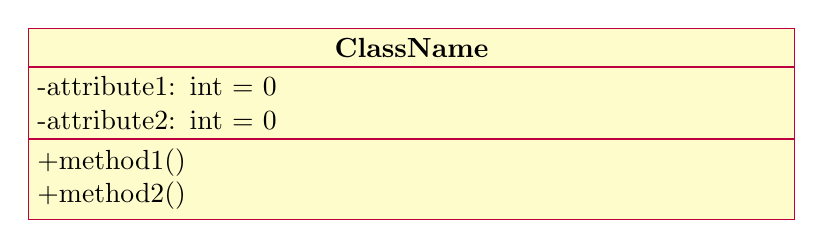
\begin{tikzpicture}
				\begin{class}[text width=9.5cm]{ClassName}{0 ,0}
					\attribute {-attribute1: int = 0}
					\attribute {-attribute2: int = 0}
					\operation {+method1()}
					\operation {+method2()}
				\end{class}
			\end{tikzpicture}
			\begin{compactitem}
				\item Eine Klasse ist der Bauplan f�r Objekte.
				\item Eine Klasse besteht aus Daten (Attribute) und den Funktionen (Methoden) auf diesen Daten.
				\item Sichtbarkeit: 
				\begin{compactitem}
					\item \lc{+} : \lc{public}
					\item \lc{-} : \lc{private}
					\item \lc{\#} : \lc{protected}
				\end{compactitem}
			\end{compactitem}
	\end{minipage} \\
	
	\begin{minipage}[t]{8 cm}	
		\subsection{�blicher Aufbau einer Klassensyntax \verweiscpp{11.1.1}}
			\lstinputlisting[language=C++,tabsize=2]{code/klassenschnittstelle.cpp} 
	\end{minipage}
	\hspace*{0.5cm}
	\begin{minipage}[t]{10 cm}		
			\subsubsection{Zugriffsschutz \verweiscpp{11.4}}
			\begin{compactitem}
				\item \lc{public} - Elemente k�nnen innerhalb und von ausserhalb der Klasse
				angesprochen werden.
					\begin{compactitem}
						\item fast alle Methoden sind \lc{public}
						\item Attribute sollen nie \lc{public} sein
					\end{compactitem}
				\item \lc{protected} - Elemente k�nnen von innerhalb der Klasse und von abgeleiteten
				Klassen angesprochen werden.
					\begin{compactitem}
						\item nur sparsam einsetzen!
					\end{compactitem}
				\item \lc{private} - Elemente k�nnen nur innerhalb der Klasse angesprochen werden.
					\begin{compactitem}
						\item grunds�tzlich f�r alle Attribute und f�r einzelne (lokale) Methoden
					\end{compactitem}
			\end{compactitem}
	\end{minipage} \\
	
	\begin{minipage}[t]{8 cm}
		\subsubsection{Operationen einer Klasse}
			Operationen eine Klasse (= Funktionen, die im Klassenrumpf definiert sind) werden als
			Elementfunktionen oder Methoden bezeichnet.	�blicherweise beginnen Elementfunktionen mit einem Kleinbuchstaben und werden in camelCase (mixedCase) notiert.	
			\lc{isEmpty();}
	\end{minipage}
	\hspace*{0.5cm}
	\begin{minipage}[t]{10 cm}	
		\subsubsection{Information Hiding}
			\begin{compactitem}
				\item Klassen exportieren generell ausschliesslich Methoden. Alle Daten sind im Innern (private-Abschnitt) verborgen, der Zugriff erfolgt �ber die so genannten Elementfunktionen.
				\item Jede Klasse besteht damit aus zwei Dateien, der Schnittstellendatei (\lc{.h}) und	der Implementierungsdatei (\lc{.cpp}).
			\end{compactitem}
	\end{minipage}	
	
			\paragraph{$friend$-Elemente \verweiscpp{11.4.2}}
				\begin{compactitem}
					\item \lc{friend} - Jede Klasse kann andere Klassen oder Funktionen zum Freund	erkl�ren. Dadurch werden die Zugriffsregeln durchbrochen.
					\item Jeder \lc{friend} darf auf alle Elemente der Klasse zugreifen.
					\item \lc{friend} ist eine \lc{C++} - Spezialit�t, welche die meisten anderen Programmiersprachen (z.B. \lc{Java}) nicht anbieten.
					\item \lc{friends}, insbesondere \lc{friend}-Klassen, k�nnen ein Anzeichen f�r schlechtes Design sein. Sie durchbrechen wichtige Prinzipien der objektorientierten Programmierung.
				\end{compactitem}					
					
		\subsubsection{Beispiel an der Klasse Rechteck}
			\begin{minipage}[t]{9cm}
				\vspace*{-0.5cm}\lstinputlisting[language=C++,tabsize=2]{code/class_rectangle_header.cpp}				
				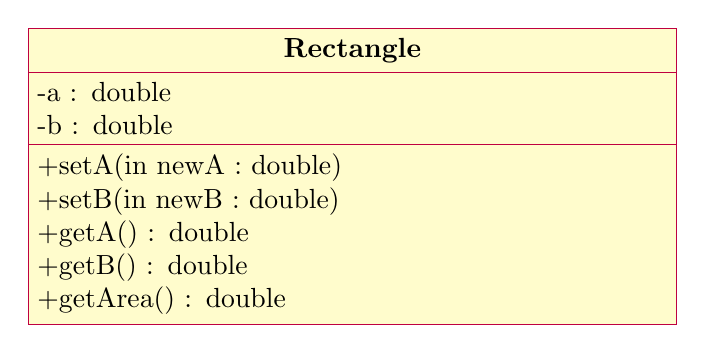
\begin{tikzpicture}
					\begin{class}[text width=8cm]{Rectangle}{0 ,0}
						\attribute{-a : double}
						\attribute{-b : double}
						\operation{+setA(in newA : double)}
						\operation{+setB(in newB : double)}
						\operation{+getA() : double}
						\operation{+getB() : double}
						\operation{+getArea() : double}
					\end{class}
				\end{tikzpicture}
			\end{minipage}
			\hspace*{0.5cm}
			\begin{minipage}[t]{9 cm}
				\vspace*{-0.5cm}\lstinputlisting[language=C++,tabsize=2]{code/class_rectangle.cpp} 
			\end{minipage} \\
			
	\begin{minipage}[t]{9cm}
		\subsection{Elementfunktionen \verweiscpp{11.2}}
			\begin{compactitem}
				\item sind Funktionen, die in der Schnittstelle der Klasse spezifiziert sind.
				\item Elementfunktionen haben vollen Zugriff auf alle Klassenelemente (auch auf
				solche, die mit \lc{private:} gekennzeichnet sind.
				\item Auf Elementfunktionen kann nur unter Bezugnahme auf ein Objekt der Klasse, bzw. mit dem Scope-Operator (\lc{::}) zugegriffen werden.
				\item Elementfunktionen sollen prinzipiell in der Implementierungsdatei (\lc{.cpp}) implementiert werden. Dem Funktionsnamen muss dabei der Klassenname gefolgt von \lc{::} vorangestellt werden. (Beispiel: \lc{int Stack::pop()})
			\end{compactitem}
	\end{minipage}
	\hspace*{0.5cm}
	\begin{minipage}[t]{9 cm}
			\subsubsection{Klassifizierung von Elementfunktionen}
				\begin{compactitem}
					\item Konstruktoren / Destruktoren
						\begin{compactitem}
							\item Konstruktor: erzeugen eines Objekts
							\item Destruktur: vernichten, freigeben eines Objekts
						\end{compactitem}
					\item Modifikatoren
						\begin{compactitem}
							\item �ndern den Zustand eines Objekts (Attribute �ndern)
						\end{compactitem}
					\item Selektoren
						\begin{compactitem}
							\item greifen nur lesend auf ein Objekt zu (immer \lc{const} definieren!)
							\item Beispiel: \lc{bool Stack::isEmpty() const;}
						\end{compactitem}
					\item Iteratoren
						\begin{compactitem}
							\item Erlauben, auf Elemente eines Objekts in einer definierten Reihenfolge	zuzugreifen
						\end{compactitem}
				\end{compactitem}
	\end{minipage} \\
	
			\subsubsection{$inline$-Funktionen \verweiscpp{11.2.1}}
				\begin{compactitem}
					\item Elementfunktionen, die innerhalb der Deklaration der Klassenschnittstelle (im	.h-File) implementiert sind, werden als (implizite) \lc{inline} - Funktionen
					behandelt.
					\item Elementfunktionen k�nnen in der Klassenimplementation explizit mit dem
					Schl�sselwort \lc{inline} gekennzeichnet werden.
					\item Implizite \lc{inline} - Funktionen verletzen zwar das Information Hiding Prinzip	und sollten deshalb grunds�tzlich vermieden werden.
					\item Jedoch: die impliziten \lc{inline} - Funktionen sind die Funktionen, die garantiert immer \lc{inline} verwendet werden (mit einigen wenigen
					Ausnahmen).
				\end{compactitem}	
		
	\vspace*{-1cm}\begin{minipage}[t]{7cm}
			\subsubsection{mutable - Attribut}
				Ein Datenelement, das nie \lc{const} werden soll (auch nicht bei \lc{const}-Elementfunktionen) kann mit \lc{mutable} gekennzeichnet werden.
				\lstinputlisting[language=C++,tabsize=2]{code/mutable.cpp}		
	\end{minipage}
	\hspace*{0.5cm}
	\begin{minipage}[t]{11 cm}			
			\subsubsection{const - Elementfunktion \verweiscpp{11.2.2}}
				\begin{compactitem}
					\item Elementfunktionen, die den Zustand eines Objekts nicht �ndern (Selektoren)
					sollen explizit mit dem Schl�sselwort \lc{const} gekennzeichnet werden.
					\item Das Schl�sselwort \lc{const} muss sowohl im Prototypen als auch in der
					Implementierung geschrieben werden.
				\end{compactitem}
				\lstinputlisting[language=C++,tabsize=2]{code/elementfunktion_const.cpp}
				
		\subsection{static - Klassenelemente \verweiscpp{11.5}}
			\begin{compactitem}
				\item Grunds�tzlich besitzt jedes Objekt einer Klasse seine eigene private Instanz
				aller Attribute einer Klasse.
				\item Wenn ein Attribut mit \lc{static} gekennzeichnet wird, dann teilen sich alle
				Objekte dieser Klasse eine einzige Instanz dieses Attributs, d.h. ein
				statisches Attribut ist nur einmal f�r alle Objekte einer Klasse im Speicher
				vorhanden.
				\item \lc{static} - Elemente befinden sich ausserhalb eines Objektkontexts.
				\item \lc{static} - Elemente k�nnen auch �ber den Klassennamen angesprochen
				werden (da sie sich im Kontext einer Klasse befinden).
			\end{compactitem}	
	\end{minipage}
			
	\subsection{$this$ - Pointer \verweiscpp{11.3}}
		Der \lc{this}-Pointer ist ein Pointer auf das eigene aktuelle Objekt, welches eine Methode aufgerufen hat.
		\lstinputlisting[language=C++,tabsize=2]{code/this_pointer.cpp}
	
	\subsection{Konstruktor (am Beispiel der Klasse TString) \verweiscpp{11.7.1}}
		\begin{minipage}[t]{9cm}
			\subsubsection{Aufgaben des Konstruktors}
				\begin{compactitem}
					\item die Neugr�ndung eines Objekts einer Klasse
					\item das saubere Initialisieren des Objekts, d.h. alle Attribute des Objekts
					m�ssen auf einen definierten Wert gesetzt werden
					\item Der Konstruktor hat in \lc{C++} denselben Namen wie die Klasse, hat keinen
					R�ckgabetyp (auch nicht \lc{void}) und kann �berladen werden. Beispiel: \lc{Stack::Stack();}
				\end{compactitem}
		\end{minipage}
		\hspace*{0.5cm}
		\begin{minipage}[t]{9cm}
			\subsubsection{Aufruf des Konstuktors}
				\begin{compactitem}
					\item Der Konstruktor soll nie explizit aufgerufen werden.
					\item Der Konstruktor wird vom System automatisch (implizit) aufgerufen, wenn
					ein Objekt erzeugt wird: \lc{Stack s;}
					\item Wenn durch den \lc{new}-Operator Speicher angefordert und erhalten wird,
					dann wird der Konstruktor vom System ebenfalls automatisch aufgerufen: \\ \lc{Stack* pS = new Stack;}
				\end{compactitem}	
		\end{minipage} 
		
		\subsubsection{Default-Konstruktor}
			\begin{minipage}[t]{13cm}
				\begin{compactitem}
					\item Der Default-Konstruktor ist der Konstruktor ohne Parameter: \\
					\lc{Stack::Stack();} \\
					Er wird immer aufgerufen, wenn bei der Objekterzeugung keine Parameter
					mitgegeben werden: \\
					\lc{Stack s;}
					\item Der Default-Konstruktor wird vom System automatisch erzeugt, wenn f�r
					eine Klasse kein Konstruktor explizit definiert ist.
					\item Der Default-Konstruktor kann selbst definiert werden.
					\begin{compactitem}
						\item Das ist insbesondere dann notwendig, wenn innerhalb des Objekts Speicher
						dynamisch alloziert werden muss (bei der Objekterzeugung).
					\end{compactitem}
				\end{compactitem}
			\end{minipage}
			\hspace*{0.5cm}
			\begin{minipage}[t]{5cm}
				\lstinputlisting[language=C++,tabsize=2]{code/constructor_default.cpp}
			\end{minipage} \\
			
		\subsubsection{Implementation/Initialisierung}
			Es gibt zwei Arten den Konstruktor zu implementieren. \\
			\begin{minipage}[t]{9cm}
				\paragraph{Implementation mit Anweisung}
					\lstinputlisting[language=C++,tabsize=2]{code/constructor_init_default.cpp}
			\end{minipage}
			\hspace*{0.5cm}
			\begin{minipage}[t]{9cm}
				\paragraph{Implementation mit Initialisierungsliste}
					\lstinputlisting[language=C++,tabsize=2]{code/constructor_init_list.cpp}
			\end{minipage} \\
			Objektinitialisierungen werden, sofern dies m�glich ist, �ber die Initialisierungsliste des Konstruktors und nicht im Anweisungsteil durchgef�hrt. (Effizienzgr�nde) \\
			
		\subsubsection{�berladen von Konstruktoren}
			\begin{minipage}[t]{6cm}
				\begin{compactitem}
					\item Der Default-Konstruktor wird implizit aufgerufen mit \\
					\lc{TString str;}
					\item Ein \lc{TString}-Objekt soll auch z.B. mit folgenden Anweisungen gegr�ndet
					werden k�nnen: \\
					\lc{TString str1 = "Hello"; // implicit call} \\
					\lc{TString str2 = TString("Guten Morgen"); // explicit call}
					\item Dazu bedarf es anderer (�berladener) Konstruktoren.
				\end{compactitem}
			\end{minipage}
			\hspace*{0.5cm}
			\begin{minipage}[t]{6cm}
				\vspace*{-0.5cm}
				\lstinputlisting[language=C++,tabsize=2]{code/constructor_overload.cpp}
			\end{minipage}
			\begin{minipage}[t]{6cm}
				\vspace*{-0.5cm}
				\lstinputlisting[language=C++,tabsize=2]{code/constructor_overload_implement.cpp}
			\end{minipage}
			
		\subsubsection{Konstruktoren und Function Casts}
			\begin{compactitem}
				\item Konstruktoren mit nur einem Parameter k�nnen dazu verwendet werden, ein
				Objekt vom Typ T aus einem anderen Objekt zu erzeugen (Typumwandlung).
				\item Beispiel:	TString soll so erweitert werden, dass dem Konstruktor eine ganze Zahl �bergeben wird und dieser daraus den entsprechenden String erzeugt.
				\lstinputlisting[language=C++,tabsize=2]{code/constructor_function_cast.cpp}
			\end{compactitem}
			
		\subsubsection{Explizite Konstruktoren}
			\begin{minipage}[t]{12cm}
				\begin{compactitem}
					\item Die implicit calls (bei Konstruktoren mit einem Parameter) \\
					\lc{TString str2 = 12345;} \\
					\lc{str2 = 789;} \\
					sind gelegentlich nicht erw�nscht.
					\item Wenn der Konstruktor mit \lc{explicit} gekennzeichnet wird, kann dieser Konstruktor	nicht mehr implizit, sondern nur explizit aufgerufen werden.
					\lstinputlisting[language=C++,tabsize=2]{code/constructor_explicit_1.cpp}
				\end{compactitem}
			\end{minipage}
			\hspace*{0.5cm}
			\begin{minipage}[t]{6cm}
					\vspace*{-0.5cm}
					\lstinputlisting[language=C++,tabsize=2]{code/constructor_explicit_2.cpp}
			\end{minipage}
			
			\vspace*{-1cm}\subsubsection{Copy-Konstruktor}
			\begin{minipage}[t]{10cm}
				\begin{compactitem}
					\item Der Copy-Konstruktor wird dazu verwendet, Objekte zu kopieren.
					\item Der Copy-Konstruktor erh�lt als Parameter immer eine konstante Referenz auf
					ein Objekt der Klasse. F�r \lc{TString} sieht er wie folgt aus: 
					\lc{TString(const TString\& s);}
				\end{compactitem}
				Der Copy-Konstruktor wird automatisch aufgerufen, wenn ...
				\begin{compactitem}
					\item ... ein Objekt mit einem anderen Objekt derselben Klasse initialisiert wird.
					\item ... ein Objekt als Wertparameter (by value) an eine Funktion �bergeben wird
					(nicht aber bei Referenzparametern).
					\item ... ein Objekt by value als Resultat einer Funktion zur�ckgegeben wird (nicht bei Referenzr�ckgabewerten).
				\end{compactitem}
				Ein Copy-Konstruktor wird nur dann benutzt, wenn ein neues Objekt erzeugt wird, aber nicht bei Zuweisungen, also �nderungen von Objekten.
				Bei Zuweisungen wird der vom System bereitgestellte Zuweisungsoperator benutzt,
				sofern kein eigener definiert wurde.
				
				\vspace*{-0.4cm}\paragraph{Shallow Copy vs. Deep Copy}
					\vspace*{-0.2cm}\begin{compactitem}
						\item Wenn f�r eine Klasse kein Copy-Konstruktor definiert wird, erzeugt das System einen Standard-Copy-Konstruktor.
						\item Dieser kopiert alle Datenelemente (memberwise assignment). Bei Pointern, welche auf den Heap zeigen, wird nur die Adresse kopiert, nicht aber der Speicher auf dem Heap. Man nennt das shallow copy. (shallow = flach).
						\item Bei einer deep copy werden auch die Speicherbereiche, auf welche Pointer
						zeigen, kopiert. Die deep copy muss in einem selbst definierten Copy-Konstruktor implementiert werden.
					\end{compactitem}
			\end{minipage}
			\hspace*{0.5cm}
			\begin{minipage}[t]{6cm}
				\vspace*{-0.5cm}
				\lstinputlisting[language=C++,tabsize=2]{code/constructor_copy.cpp}
				\lstinputlisting[language=C++,tabsize=2]{code/constructor_copy_2.cpp}
			\end{minipage} \\
			
			\begin{minipage}[t]{9cm}
				\vspace*{-0.3cm}\paragraph{Shallow-Copy}
					\vspace*{-0.5cm}\includegraphics[width=1\textwidth]{pics/shallow_copy.jpg}
			\end{minipage}
			\hspace*{0.5cm}
			\begin{minipage}[t]{9cm}
				\vspace*{-0.3cm}\paragraph{Deep-Copy}
					\vspace*{-0.5cm}\includegraphics[width=1\textwidth]{pics/deep_copy.jpg}
			\end{minipage}
			
	\vspace*{-0.1cm}\subsection{Destruktor \verweiscpp{11.7.2}}
		\vspace*{-0.4cm}\begin{minipage}[t]{7cm}
			\subsubsection{Aufgaben des Destruktors}
				\begin{compactitem}
					\item die vollst�ndige Zerst�rung eines nicht mehr ben�tigten Objekts
					\item das saubere Entfernen eines Objekts
					\item die h�ufigste Aufgabe ist die Freigabe von nicht mehr ben�tigtem Speicher auf dem Heap
					\item sehr h�ufig (wenn kein Speicher auf dem Heap vorhanden ist) wird kein
					Destruktor definiert, da das System dann automatisch aufr�umt
				\end{compactitem}
		\end{minipage}
		\hspace*{0.5cm}
		\begin{minipage}[t]{11cm}
			\subsubsection{Eigenschaften des Destruktors}
				\begin{compactitem}
					\item Destruktoren haben keine Argumente und keinen R�ckgabetyp
					\item Ihr Name besteht aus dem Klassennamen mit vorgestellter Tilde. Der
					Destruktor soll meist virtual deklariert werden (wenn es einen Destruktor
					braucht): \lc{virtual ~TString();}					
					\item Destruktoren werden automatisch aufgerufen, wenn der G�ltigkeitsbereich des definierten Objektes ausl�uft 
					\item Die Reihenfolge des Aufrufs der Destruktoren ist umgekehrt wie die der
					Konstruktoren
					\item Nicht definierte Destruktoren werden automatisch erzeugt
				\end{compactitem}	
		\end{minipage}
			
	\subsection{Kanonische Form von Klassen \verweiscpp{11.7.5}}
		\begin{compactitem}
			\item Als kanonische Form einer Klasse bezeichnet man jene Form, die es erlaubt,
			eine Klasse wie einen "normalen" Datentyp zu benutzen. Dies ist f�r alle Klassen anzustreben.
			\item Dazu m�ssen drei Bedingungen erf�llt sein:
			\begin{compactitem}
				\item Ein korrekter Default-Konstruktor, plus evtl. weitere Konstruktoren m�ssen
				vorhanden sein
				\item Wenn die Klasse dynamische Daten enth�lt, braucht es auch einen
				Zuweisungsoperator und einen Copy-Konstruktor
				\item Ein (virtueller) Destruktor garantiert die korrekte Zerst�rung von Objekten
			\end{compactitem}
		\end{compactitem}
		
	\subsection{Benutzerdefinierte Typumwandlung \verweiscpp{11.7.6}}
		Wenn zwei ganze Zahlen unterschiedlichen Typs (z.B. \lc{int} und \lc{short}) addiert werden, so ist der Additionsoperator vom System f�r folgende Varianten	definiert:
		\begin{compactitem}
			\item \lc{int+int}
			\item \lc{int+short}
			\item \lc{short+int}
			\item \lc{short+short}
		\end{compactitem}
		Wenn nun eine neue Klasse \lc{VeryLargeInt} eingef�hrt wird, so sind die Operatoren f�r diese Klasse noch nicht definiert. Nur schon f�r den Additionsoperator zwischen \lc{VeryLargeInt} und \lc{int} m�ssten folgende Varianten definiert werden:
		\begin{compactitem}
			\item \lc{int+VeryLargeInt}
			\item \lc{VeryLargeInt+int}
			\item \lc{VeryLargeInt+VeryLargeInt}
		\end{compactitem}
		Dasselbe gilt auch f�r alle weiteren Operatoren. F�r die Grundoperatoren \lc{+}, \lc{-}, \lc{*},
		\lc{/}, \lc{+=}, \lc{-=}, \lc{*=}, \lc{/=} m�ssten somit 24 Operatoren definiert werden. \\
		Die einfachere Variante ist, wenn f�r jeden Typ eine Typumwandlung definiert
		wird. Somit braucht es pro Typ eine Umwandlungsfunktion, die Operatoren arbeiten
		anschliessend nur noch mit der Klasse \lc{VeryLargeInt}.
		\begin{compactitem}
			\item \lc{VeryLargeInt+VeryLargeInt}
		\end{compactitem}
		F�r die Grundoperatoren \lc{+}, \lc{-}, \lc{*},	\lc{/}, \lc{+=}, \lc{-=}, \lc{*=}, \lc{/=} m�ssten nur noch die 8 Operatoren definiert werden. Zus�tzlich m�sste noch die Typumwandlung von jedem Typ (\lc{short}, \lc{int}, etc.) in \lc{VeryLargeInt} definiert werden. \\
		H�ufig werden Typumwandlungen aber auch mit Hilfe von Konstruktoren implementiert:
		\lc{VeryLargeInt(int);}
		
	\subsection{�berladen von Operatoren \verweiscpp{11.7.3}}
		Operatoren (z.B. +, ==, etc.) k�nnen wie Funktionen �berladen werden.
		
		\subsubsection{�berladbare Operatorfunktionen in C++}
			\begin{minipage}[c]{2.2 cm}
	 			\begin{compactitem}
	 				\item \lc{new}
	 				\item \lc{delete}				
	 				\item \lc{new[ ]}				
	 				\item \lc{delete[ ]} 	
	 				\item \lc{+}
	 				\item \lc{-}							
	 			\end{compactitem}
 			\end{minipage}
 			\begin{minipage}[c]{2.3 cm}
	 			\begin{compactitem}	
	 				\item \lc{*}
	 				\item \lc{/}			
	 				\item \lc{\%}
	 				\item \lc{\textasciicircum}
	 				\item \lc{\&}	
	 				\item \lc{|}		
	 			\end{compactitem}
 			\end{minipage}
 			\begin{minipage}[c]{2.2 cm}
	 			\begin{compactitem}	
	 			 	\item \lc{\textasciitilde}
	  			 	\item \lc{!}	
	 			 	\item \lc{=} 			 	
	 			 	\item \lc{<} 	
	 			 	\item \lc{>}	 		 	
	 			\end{compactitem}
 			\end{minipage}
 			\begin{minipage}[c]{2.2 cm}
	 			\begin{compactitem}	
	 			 	\item \lc{+=}			 	
	 			 	\item \lc{-=}			 	
	 			 	\item \lc{*=}		
	 			 	\item \lc{/=}	
	 			 	\item \lc{\%=}		 	
	 			\end{compactitem}
	 		\end{minipage}
 			\begin{minipage}[c]{2.2 cm}
	 			\begin{compactitem} 
	 			 	\item \lc{\textasciicircum=}			 	
	 			 	\item \lc{\&=} 		 	
	 			 	\item \lc{|=}			 	
	 			 	\item \lc{<<}		
	 			 	\item \lc{>>}	 	
	 			\end{compactitem}
	 		\end{minipage}
 			\begin{minipage}[c]{2.2 cm}
	 			\begin{compactitem}		 
	 			 	\item \lc{>>=} 			 	
	 			 	\item \lc{<<=}			 	
	 			 	\item \lc{==} 			 	
	 			 	\item \lc{!=}
	 			 	\item \lc{<=}	
	 			\end{compactitem}
	 		\end{minipage}
 			\begin{minipage}[c]{2.2 cm}
	 			\begin{compactitem}		 	
	 			 	\item \lc{>=} 		 	
	 			 	\item \lc{\&\&} 			 	
	 			 	\item \lc{||} 			 	
	 			 	\item \lc{++} 		
	 			 	\item \lc{--}	 	
	 			\end{compactitem}
	 		\end{minipage}
 			\begin{minipage}[c]{2.4 cm}
	 			\begin{compactitem}		 	
	 			 	\item \lc{,} 			 	
	 			 	\item \lc{->*}	
	 			 	\item \lc{->}		 	
	 			 	\item \lc{()}
	 			 	\item \lc{[ ]}
	 			\end{compactitem}
	 		\end{minipage}
	 		
		\subsubsection{Randbedingungen}
			\begin{compactitem}
				\item Die Anzahl der Operanden (Argumente) muss gleich sein wie beim urspr�nglichen Operator.
				\item Die Priorit�t des �berladenen Operators kann nicht �ndern.
				\item Neue Operatoren k�nnen nicht eingef�hrt werden.
				\item Default-Argumente sind bei Operatoren nicht m�glich.
			\end{compactitem}
			
		\begin{minipage}[t]{9cm}	
			\subsubsection{Operator Overloading als Elementfunktion}
				Der neu definierte Operator wird als Elementfunktion implementiert. Damit ist
				der Zugriff auf \lc{private} und \lc{protected} Attribute der Klasse m�glich.
				\lstinputlisting[language=C++,tabsize=2]{code/operator_overloading_element.cpp}
				Zwingend als Elementfunktion zu implementieren sind: \\
				Zuweisungsoperator \lc{=}, Indexaufruf \lc{[ ]}, Funktionsaufruf \lc{()} und Zeigeroperator \lc{->}			
		\end{minipage}
		\hspace*{0.5cm}
		\begin{minipage}[t]{9cm}	
			\subsubsection{Operator Overloading als normale Funktion}
				Die Operatorfunktionen werden meist als normale Funktion implementiert. Dadurch besteht jedoch kein Zugriff mehr auf die \lc{private} und \lc{protected} Elemente der Klasse. Die Operatorfunktion muss deshalb als \lc{friend} deklariert werden.
				\lstinputlisting[language=C++,tabsize=2]{code/operator_overloading_normal.cpp}
		\end{minipage} \\
		
	\subsection{Strukturen und Unionen \verweisboth{11}{11.8.2}}
		\subsubsection{Strukturen \verweisc{11.1}}
			\paragraph{Eigenschaften}
				\begin{compactitem}
					\item Daten, welche logisch zusammengeh�ren, k�nnen zusammengenommen werden
					\item Die Struktur ist ein zusammengesetzter Datentyp, sie setzt sich aus den Feldern zusammen
					\item Die einzelnen Felder der Strukturen k�nnen (m�ssen aber nicht) unterschiedliche Typen haben
					\item Jedes Feld wird mit einem innerhalb der Struktur eindeutigen Namen versehen $\rightarrow$ Strukturspezifische Pr�fixe f�r die Feldnamen (z.B. \lc{Angestellter\_Vorname}) sind deshalb sinnlos. 
				\end{compactitem}
			
			\begin{minipage}[t]{10 cm}
				\paragraph{Definition von Strukturtypen}
					\vspace*{-0.2cm}
					\lstinputlisting[language=C,tabsize=2]{code/strukturen1.c}
					\vspace*{0.3cm}
					\begin{compactitem}
						\item \lc{StructName} kann frei gew�hlt werden
						\item \lc{struct StructName} ist hier ein selbst\\ definierter Typ, der weiter verwendet werden kann
						\item Der Datentyp ist definiert durch den Inhalt der\\ geschweiften Klammer
						\item Der Feldtyp kann wiederum eine Struktur sein
					\end{compactitem}
			\end{minipage}
			\hspace*{0.5cm}	
			\begin{minipage}[t]{8 cm}
				\paragraph{Beispiel}
					\vspace*{-0.2cm}
					\lstinputlisting[language=C,tabsize=2]{code/strukturen2.c}
			\end{minipage}
		
			\paragraph{Beispiele f�r die Definition von Strukturvariablen}
				\vspace*{-0.2cm}
				\lstinputlisting[language=C,tabsize=2]{code/strukturen3.c}
				\vspace*{0.3cm}	
					
			\paragraph{Operationen auf Strukturvariablen}
				\begin{compactitem}
					\item Zuweisung: liegen zwei Strukturvariablen a und b vom gleichen Strukturtyp vor, so kann der Wert der einen Variablen der anderen zugewiesen werden \lc{$\rightarrow$ a=b;}
					\item Ermittlung der Gr�sse der Struktur: mit \lc{sizeof}-Operator
					\item Ermittlung der Adresse der Strukturvariablen: mit Adressoperator \lc{\&}
				\end{compactitem}
				
			\paragraph{Zugriff auf eine Strukturvariable und deren Felder}
				\begin{minipage}[t]{9cm}
					Der Zugriff auf ein Feld einer Strukturvariablen erfolgt �ber
					\begin{compactitem}
						\item den Namen der Strukturvariablen,
						\item gefolgt von einem Punkt
						\item und dem Namen des Feldes 
					\end{compactitem}	
				\end{minipage}
				\hspace*{0.5cm}
				\begin{minipage}[t]{9cm}		
					... wenn der Zugriff �ber einen Pointer erfolgt, �ber
					\begin{compactitem}
						\item den Namen des Pointers,
						\item gefolgt von einem Pfeil (--\textgreater)
						\item und dem Namen des Feldes 
					\end{compactitem}
				\end{minipage}
							
			\paragraph{Beispiele f�r den Zugriff auf eine Strukturvariable}
				\vspace*{-0.2cm}
				\lstinputlisting[language=C,tabsize=2]{code/strukturen4.c}
				\vspace*{0.3cm}

			\begin{minipage}[c]{8 cm}
				\paragraph{Lage im Speicher}
					\begin{compactitem}
						\item Die Felder einer Strukturvariablen werden nacheinander gem�ss der Definition in den Speicher gelegt.
						\item Gewisse Datentypen verlangen unter Umst�nden, dass sie auf eine Wortgrenze (gerade Adresse) gelegt werden. Dies nennt man Alignment.
						\item Durch das Alignment kann es vorkommen, dass einzelne Bytes nicht verwendet werden, d.h. im Speicher ausgelassen werden.
						\item Die Gr�sse einer Strukturvariablen kann nicht durch Addieren der Gr�ssen der Felder ermittelt werden, nur $sizeof()$ liefert den genauen Wert
					\end{compactitem}
			\end{minipage}
			\hspace*{2cm}
			\begin{minipage}[c]{7 cm}
				\includegraphics[width=0.5\textwidth]{pics/alignment.png}
			\end{minipage}
			\hspace*{-3cm}	
			\begin{minipage}[c]{3 cm}
				\lstinputlisting[language=C,tabsize=2]{code/strukturen5.c}
				\vspace*{0.5cm}
				Das int-Feld zahl muss auf einer geraden Adresse beginnen!
			\end{minipage}
			
			\paragraph{�bergabe und R�ckgabe von Strukturvariablen}
				\begin{compactitem}
					\item Strukturvariablen k�nnen komplett an Funktionen �bergeben werden
					\item Der R�ckgabetyp einer Funktion kann eine Struktur sein. Dabei wird die Strukturvariable direkt komplett �bergeben
					\item Zu beachten ist der Kopieraufwand bei der �bergabe, bzw. R�ckgabe eines Wertes. In der Praxis soll deshalb mit Pointern gearbeitet werden!
					\lstinputlisting[language=C,tabsize=2]{code/strukturen7.c} 
				\end{compactitem}
			
		\begin{minipage}[t]{9cm}
			\paragraph{Initialisierung einer Strukturvariablen}
				Eine Initialisierung einer Strukturvariablen kann direkt bei der Definition der Strukturvariablen mit Hilfe einer Initialisierungsliste durchgef�hrt werden (Reihenfolge beachten). Nat�rlich muss der Datentyp \lc{struct Angestellter} bereits bekannt sein. 
				\lstinputlisting[language=C,tabsize=2]{code/strukturen6.c} 	
		\end{minipage}
		\hspace*{0.5cm}
		\begin{minipage}[t]{10cm}					
			\subsubsection{Unions \verweisboth{11.2}{11.8.2}}
				\paragraph{Eigenschaften}
					\begin{compactitem}
						\item �hnlich wie Struktur
						\item beinhaltet auch mehrere Felder unterschiedlichen Typs
						\item im Gegensatz zur Struktur ist aber nur ein einziges Feld jeweils aktiv (abh�ngig vom Typ)
						\item Die Gr�sse einer Union ist so gross wie das gr�sste Feld der Union
						\item Bei der Union sind dieselben Operationen wie bei einer Struktur definiert 
					\end{compactitem}
					
					\paragraph{Definition von Uniontypen}											
						\begin{minipage}[t]{5.5cm}
							\begin{compactitem}
								\item \lc{UnionName} kann frei gew�hlt werden
								\item \lc{union UnionName} ist ein hier selbst definierter Typ, \\der weiter verwendet werden kann
								\item Der Datentyp ist definiert durch den Inhalt der \\geschweiften Klammer
								\item Der Feldtyp kann wiederum eine Union oder \\auch eine Struktur sein
							\end{compactitem}
						\end{minipage}	
						\hspace*{0.5cm}
						\begin{minipage}[t]{3.5cm}
								\vspace*{-0.2cm}
								\lstinputlisting[language=C,tabsize=2]{code/unions1.c}
						\end{minipage}	
		\end{minipage} 
		
		\begin{minipage}[t]{5 cm}
				\paragraph{Beispiel}
					\vspace*{-0.4cm}
					\lstinputlisting[language=C,tabsize=2]{code/unions2.c}
					\includegraphics[width=0.7\textwidth]{pics/union.png}
		\end{minipage}
		\hspace*{0.5cm}	
		\begin{minipage}[t]{13 cm}
		\subsubsection{Allgemeines zu Strukturen und Unions}
			\paragraph{Codierstil}
				\begin{compactitem}
					\item \lc{Strukturname} und \lc{Unionname} mit einem grossen Buchstaben beginnen!\\
					\lc{struct Angestellter;}\\
					\lc{union Vario;}
					\item Struktur- und Unionvariablen mit einem kleinen Buchstaben beginnen
					\item Bei Feldern von Strukturen und Union soll kein Pr�fix bei den Feldnamen verwendet werden
				\end{compactitem}
				
			\paragraph{Vorsicht bei Unions}	
				\begin{compactitem}
					\item Der Programmierer muss verfolgen, welcher Typ jeweils in der Union gespeichert ist. Der Datentyp, der entnommen wird, muss der sein, der zuletzt gespeichert wurde. 
				\end{compactitem}
		\end{minipage}			
	
	\section{Templates}
	\subsection{Motivation \verweiscpp{12.1}}
		Wesentliche Vorteile von Templates sind:
		\begin{compactitem}
			\item Single-Source-Prinzip: F�r x Varianten derselben Datenstruktur existiert genau eine Version des Sourcecodes, der ge�ndert und gewartet werden muss.
			\item H�here Wiederverwendbarkeit: Klassen-Templates sind bei geeigneter Wahl ihrer Parameter allgemein einsetzbar und einfach wiederverwendbar.
			\item Statische Bindung: Die Bindung zur �bersetzungszeit hat in Bezug auf Typsicherheit und Fehlererkennung zweifellos grosse Vorteile gegen�ber generischen C-L�sungen mit $void*$-Zeigern, aber zum Teil auch gegen�ber typisch objektorientierten Varianten wie sie zum Beispiel in Smalltalk �blich sind.
			\item Dead Code: Traditionelle Bibliotheken belegen Speicher unabh�ngig davon, ob eine
			einzelne Funktion wirklich verwendet wird. Dies kann zu Dead Code f�hren,
			d.h. zu Code, der niemals ausgef�hrt wird.
		\end{compactitem}
		
	\subsection{Funktions-Templates \verweiscpp{12.2}}
		\begin{compactitem}
			\item Templates verwenden den Typ als Variable.
			\item Die Algorithmen k�nnen unabh�ngig vom Typ (generisch) implementiert
			werden.
			\item Templates sind keine Funktionsdefinitionen, sie beschreiben dem Compiler
			nur, wie er den Code definieren soll, d.h. der Compiler nimmt den konkret
			verwendeten Typ, setzt diesen in das Template ein und compiliert den so
			erhaltenen Code.
			\item Die Bindung zum konkreten Typ geschieht bereits zur Compiletime (early
			binding), sobald bekannt ist, mit welchem Typ das Template aufgerufen
			(benutzt) wird.
		\end{compactitem}
		
		\subsubsection{Syntax}
			\begin{minipage}[t]{10.5cm}
				\begin{compactitem}
					\item Vor den Funktionsnamen wird das Schl�sselwort template, gefolgt von einer
					in spitzen Klammern eingeschlossenen Parameterliste gestellt.
					\item Die Parameterliste enth�lt eine (nicht leere) Liste von Typ- und
					Klassenparametern, die mit dem Schl�sselwort class oder typename
					beginnen. Die einzelnen Parameter werden mit Komma getrennt.
				\end{compactitem}
			\end{minipage}
			\hspace*{0.5cm}
			\begin{minipage}[t]{7cm}
				\vspace*{-0.5cm}\lstinputlisting[language=C++,tabsize=2]{code/template_syntax.cpp}
			\end{minipage} \\
		
		\begin{minipage}[t]{11cm}
			\subsubsection{$inline$ bei Templates}
				$inline$ muss zwischen $template$ und dem Returntyp stehen.
				Achtung: Bei Verwendung von $inline$ speziell zusammen mit Templates besteht die Gefahr von Code Bloat.
							
			\subsubsection{Auspr�gung \verweiscpp{12.2.1}}
				\begin{compactitem}
					\item Sobald ein Typ in einem Funktions-Template verwendet wird, erkennt der
					Compiler, dass es sich um ein Template handelt und pr�gt es f�r diesen Typ aus
					(implizite Auspr�gung).
					\item F�r die Aufl�sung werden nur die Funktionsparameter betrachtet, der
					R�ckgabetyp wird nicht ausgewertet.			
				\end{compactitem}
				\lstinputlisting[language=C++,tabsize=2]{code/template_auspraegung.cpp}
				
			\subsubsection{Explizite Qualifizierung}
				\begin{compactitem}
					\item Funktions-Templates k�nnen explizit mit einem Typ qualifiziert werden.		
				\end{compactitem}
				\lstinputlisting[language=C++,tabsize=2]{code/template_explizit.cpp}
		\end{minipage}
		\hspace*{0.5cm}
		\begin{minipage}[t]{7cm}			
			\subsubsection{�berladen \verweiscpp{12.2.2}}
				\begin{compactitem}
					\item Funktions-Templates k�nnen mit anderen Funktionstemplates und auch mit
					normalen Funktionen �berladen werden.
					\item Namensaufl�sung:
					\begin{compactitem}
						\item Compiler geht Liste der m�glicherweise passenden Funktions-Templates durch und erzeugt die entsprechenden Template-Funktionen.
						\item Ergebnis ist eine Reihe von (eventuell) passenden Template-Funktionen, erg�nzt durch die vorhandenen normalen Funktionen.
						\item Aus dieser ganzen Auswahl wird die am besten passende Funktion ausgew�hlt.
					\end{compactitem}	
				\end{compactitem}
		\end{minipage}
		
	\subsection{Klassen-Templates \verweiscpp{12.3}}
		\begin{minipage}[t]{7 cm}
			\subsubsection{Definition \verweiscpp{12.3.1}}
				\begin{compactitem}
					\item Klassen-Templates sind mit Typen oder Konstanten parametrisierbare Klassen.
					\item Im Gegensatz zu Funktions-Templates k�nnen in Klassen-Templates auch die
					Attribute der Klassen mit variablen Typen ausgestattet sein.
					\item Ein Klassen-Template kann auch von Ausdr�cken abh�ngig sein. Diese Ausdr�cke m�ssen aber zur Compiletime aufgel�st werden k�nnen.
				\end{compactitem}
				
			\subsubsection{Syntax}
				\begin{compactitem}
					\item Die Syntax ist analog zu den Funktions-Templates.
					\item Vor die Klassendeklaration wird das Schl�sselwort $template$, gefolgt von
					einer in spitzen Klammern eingeschlossenen Parameterliste gestellt.
					\item Die Parameterliste enth�lt eine (nicht leere) Liste von Typ- und
					Klassenparametern, die mit dem Schl�sselwort $class$ oder $typename$
					beginnen oder auch von Ausdr�cken. Die einzelnen Parameter werden mit Komma getrennt.
				\end{compactitem}
		\end{minipage}
		\hspace*{0.5cm}
		\begin{minipage}[t]{11 cm}
			\lstinputlisting[language=C++,tabsize=2]{code/template_class.cpp}
		\end{minipage}
		
	\subsection{Klassen-Templates und getrennte �bersetzung}
		\begin{minipage}[t]{9 cm}
			\subsubsection{M�glichkeit 1}
				\includegraphics[width=1\textwidth]{pics/template_klasse_1.jpg}
		\end{minipage}
		\hspace*{0.5cm}
		\begin{minipage}[t]{9 cm}
			\subsubsection{M�glichkeit 2}
				\includegraphics[width=1\textwidth]{pics/template_klasse_2.jpg}
		\end{minipage}	
	
	\section{Vererbung (Inheritance)}
	Vererbung ist ein Konzept, das es erlaubt, neue Klassen auf Basis von alten Klassen zu definieren. Die neuen (Unter-, Sub-) Klassen besitzen, ohne Eingriffe in den
	Sourcecode der bereits bestehenden (Ober-, Basis-, Super-) Klassen, all deren Eigenschaften, sie $erben$ deren Verhalten und Daten. Den Vorgang der Vererbung nennt man $Ableiten$.\linebreak
	\begin{minipage}[t]{7 cm}
		\subsection{Einsatz der Vererbung \verweiscpp{13.1}}
		\begin{compactitem}
			\item Bestehende Klassen erweitern (zus�tzliche Attribute und Elementfunktionen)
			\item Bestehende Methoden einer Basisklasse �ndern (�berschreiben)
			\item Einsatz nur wenn eine \textbf{IST-EIN (\phantom{}is a")} Beziehung besteht (z.B. Baum \textbf{ist eine} Pflanze, Blume \textbf{ist eine} Pflanze)
			\linebreak
		\end{compactitem}
		\includegraphics[width=1\textwidth]{pics/bsp_Vererbung.jpg}
		\subsection{Ableiten einer Klasse \verweiscpp{13.2}}
			Der Syntax der Ableitung einer Klasse ist oben aufgef�hrt. Als weiteres Beispiel ist im Anhang das Beispiel des ComicCharacters und SuperHero eingef�gt. SuperHero \textbf{ist ein} ComicCharacter.
			\begin{compactitem}
				\item friend-Beziehungen werden nicht vererbt
				\item Ein Objekt einer Oberklasse kann Objekte einer beliebigen Unterklasse aufnehmen
				\item Ein Objekt einer Unterklasse kann keine Objekte der Oberklasse aufnehmen
				\item Ein Objekt einer vererbten Klasse enth�lt alle Teile der Basisklasse und zus�tzlich noch die spezifischen eigenen Teile.
				\item Das Objekt ist somit mindestens so gross wie jenes der Basisklasse (es gibt keine Vererbung $by$ $reference$)
				\linebreak
			\end{compactitem}
			\lstinputlisting[language=C++,tabsize=2]{code/substitutionsprinzip.cpp}
	\end{minipage}	
	\hspace*{0.5cm}
	\begin{minipage}[t]{11.5 cm}
	\subsection{Zugriff auf Elemente der Basisklasse \verweiscpp{13.6}}
		\textbf{Bei Vererbung mit public (Normalfall):}
			\begin{compactitem}
				\item Zugriff m�glich auf alle public- und protected- Elemente der Basisklasse, die Zugriffsrechte 
				(public, protected) der Basisklasse werden in der abgeleiteten Klasse beibehalten
				\linebreak
			\end{compactitem}
		\textbf{Bei Vererbung mit protected:}
			\begin{compactitem}
				\item Zugriff m�glich auf alle public- und protected- Elemente der Basisklasse, die Zugriffsrechte 
				von public und protected der Basisklasse werden in der abgeleiteten Klasse zu protected
				\linebreak
			\end{compactitem}
		\textbf{Bei Vererbung mit private:}
			\begin{compactitem}
				\item Zugriff m�glich auf alle public- und protected- Elemente der Basisklasse, die Zugriffsrechte 
				von public und protected der Basisklasse werden in der abgeleiteten Klasse zu private
				\linebreak
			\end{compactitem}
		\textbf{Bei allen drei: kein Zugriff auf private-Elemente der Basisklasse}
		\lstinputlisting[language=C++,tabsize=2]{code/privateFehler.cpp}
	\subsection{Slicing Problem \verweiscpp{13.3}}
		Links: Beim Kopieren werden nur die ComicCharacter-Teile ber�cksichtigt. Durch das Kopieren wird alles �berfl�ssige weggeschnitten, �brig bleibt ein reines ComicCharacter Objekt im Fall von s f�hrt dies dazu, dass die erweiterten SuperHero Daten und Funktionen verloren gehen.\newline
		Rechts: Hier wird dank des Referenzparameters der gesamte Superheld ausgegeben.\newline
		\includegraphics[width=0.8\textwidth]{pics/SlicingProblem.jpg}
	\subsection{Vererbung und G�ltigkeitsbereiche \verweiscpp{13.4}}
		\includegraphics[width=0.5\textwidth]{pics/zugriffVererbung.jpg}
	\end{minipage}	
\newpage
	\subsection{Elementfunktionen bei abgeleiteten Klassen \verweiscpp{13.5}}
	\begin{minipage}[t]{12 cm}
    	\subsubsection{Konstruktoren}
    	In einem Konstruktor m�ssen alle Elemente eines Objekts (auch die ererbten) initialisiert werden. Folgendes Beispiel zeigt die direkte Initialisierung aller Elemente. Vor allem bei grossen oder mehreren Klassen ist dies nicht zielf�hrend. Stattdessen wird das Chaining Prinzip angewandt. Falls kein Aufruf eines Basislklassen-Konstruktors in der Initialisierungsliste eines Konstruktors erscheint, so f�gt der Compiler automatisch den Default-Konstruktor der Basisklasse ein.
   		\lstinputlisting[language=C++,tabsize=2]{code/initVererbungKonstruktor.cpp}
   		\subsubsection{Chaining}
   		Jede Klasse erledigt nur die eigenen Aufgaben. Aufgaben, die ererbte Methoden �bernehmen k�nnen, werden diesen delegiert (Aufruf der jeweiligen Konstruktoren)\newline
   		\textbf{Wichtig: die Elemente der Basisklasse m�ssen immer als erste initialisiert werden}
    \lstinputlisting[language=C++,tabsize=2]{code/initVererbungChaining.cpp}
	\end{minipage} \hspace*{0.5cm}
	\begin{minipage}[t]{6.5 cm}
		\subsubsection{Copy-Konstruktor}
			\begin{compactitem}
				\item Wenn kein Copy Constructor explizit definiert wird, so erzeugt das System einen
				\item Darin wird immer (ebenfalls automatisch) zuerst der Copy Constructor der Basisklasse aufgerufen
				\linebreak
			\end{compactitem}
		\subsubsection{Destruktor}
			\begin{compactitem}
				\item Auch Destruktoren werden nach dem Chaining-Prinzip aufgebaut
				\item Jede Klasse k�mmert sich um die eigenen Attribute und �berl�sst jene der
				Basisklasse auch der Basisklasse
				\item Destruktoren m�ssen nie explizit aufgerufen werden. Der Destruktor der
				Basisklasse wird \textbf{am Schluss} des Destruktors immer automatisch aufgerufen
				\linebreak
		\end{compactitem}
		
	\end{minipage}

    
	
	
	\section{Polymorphismus / Mehrfachvererbung / RTTI}
   	\begin{flushleft}
   	Dieses Kapitel beschreibt die dynamischen objektorientierten Sprachmerkmale von C++. Erst durch diese wird C++ zu einer echten objektorientierten Programmiersprache.
   	\end{flushleft}
	\begin{minipage}[t]{8 cm}
		\subsection{Polymorphismus \verweiscpp{14.1}}
			\subsubsection{dynamische vs. statische Bindung}
			Werden von einer Kasse A die Klassen B und C abgeleitet, so k�nnen Objekte vom Typ $Zeiger auf A$ auch auf B- oder C-Objekte verweisen. Implementieren alle drei Klassen eine Operation foo jeweils verschieden so bewirkt die Anweisung
			\lstinputlisting[language=C++,tabsize=2]{code/foo_poly.cpp}
			in normalen Programmiersprachen den Aufruf von $A::foo()$. Dabei wird bereits zur �bersetzungszeit (so fr�h wie m�glich; Early Binding) vom Compiler die Funktion $foo$ der Klasse A eingebunden. Diese Art des Bindens wird statische Bindung (static binding) genannt, da sie unver�nderbar ist. Die Variable $anAPointer$ kann in C++ auch f�r Objekte der Klasse B oder C stehen. \linebreak
			In echten objektorientierten Programmiersprache wird der obige Aufruf nicht zur �bersetzungszeit, sondern erst zur Laufzeit gebunden (dynamische Bindung, dynamic Binding). Beim Aufruf von \lstinputlisting[language=C++,tabsize=2]{code/foo_poly.cpp} wird der Typ des Objekts untersucht. In Abh�ngigkeit davon wird die Methode $A::foo$, $B::foo$ oder $C::foo$ aufgerufen. Dieses dynamische Verhalten wird als Polymorphismus bezeichnet. Damit dynamisch (zur Laufzeit) die verschiedenen Funktionen foo aufgerufen werden k�nnen, m�ssen diese Funktionen $virtual$ sein. \linebreak
	\end{minipage}\hspace*{0.5cm}
	\begin{minipage}[t]{10.5 cm}
		\subsection{Virtuelle Elementfunktionen \verweiscpp{14.2}}
			Virtuelle Elementfunktionen sind spezielle Funktionen, die nicht zur �bersetzungs- sondern zur Laufzeit gebunden werden. Es wird erst beim Auruf der Funktion entschieden, welche tats�chlich ausgef�hrt wird $A::foo$, $B::foo$ oder $C::foo$
				\begin{compactitem}
					\item Funktionen, die dynamisch gebunden werden, muss bei der Deklaration das Schl�sselwort virtual vorangestellt werden (zwingend!).
					In der abgeleiteten Klasse soll (muss aber nicht) die Funktion auch mit virtual gekennzeichnet werden. Dies sieht wie folgt aus:
						\lstinputlisting[language=C++,tabsize=2]{code/virtual.cpp}
					\item Faustregel: Eine Funktion sollte als virtual deklariert werden, wenn sie in der abgeleiteten Klasse neu definiert (�berschrieben) wird, sonst nicht!
					\item Achtung: nicht mit Funktions�berladung (gleicher Name aber unterschiedliche Signatur) verwechseln
					\item Die neue (�berschriebene) Methode muss dieselbe Signatur wie die Methode der Basisklasse haben. Sonst wird neue Methode eingef�hrt.
					\linebreak
				\end{compactitem}
	\end{minipage}
	\begin{minipage}[t]{6.5 cm}
	Im Beispiel rechts wird die Verwendung klar:
			\begin{compactitem}
				\item Der statische Datentyp bezeichnet den Datentyp bei der Deklaration. Im Beispiel: a ist ein Array von Pointer auf Article
				\item Der dynamische Datentyp bezeichnet den effektiven Datentyp zur Laufzeit Im Beispiel: a[0] ist ein Pointer auf Book, a[1] ein Pointer auf CD, etc.
			\end{compactitem}
	\end{minipage}
	\hspace*{0.5cm}
	\begin{minipage}[t]{12 cm}
	test\linebreak
		\includegraphics[width=1\textwidth]{pics/bsp_Webshop.jpg}
	\end{minipage}
\newpage
	\subsubsection{Aufruf von virtuelle Elementfunktionen \verweiscpp{14.2.2}}
	\begin{minipage}[t]{9 cm}
		Eine dynamische Methodenaufl�sung erfolgt �ber Zeiger oder Pointer:
		\lstinputlisting[language=C++,tabsize=2]{code/dynamic_call.cpp}
	\end{minipage}\hspace*{0.5cm}
	\begin{minipage}[t]{9 cm}
		Ein Aufruf mit einem Objekt und der Punktnotation wird statisch aufgel�st:
		\lstinputlisting[language=C++,tabsize=2]{code/static_call.cpp}
		Dies kommt daher, dass ein echtes Objekt sein Typ nicht ver�ndern kann (nicht polymorph) und der Compiler somit schon zur �bersetzungszeit entscheidet welche Funktion aufgerufen wird.
	\end{minipage}
	\begin{flushleft}
		Eine statische Aufl�sung wird auch erzwungen, wenn der G�ltigkeitsbereich explizit angegeben wird:
	\end{flushleft}
		\lstinputlisting[language=C++,tabsize=2]{code/static_call2.cpp}
	\begin{flushleft}
		Wichtig ist auch: innerhalb von Konstruktoren und Destruktoren \textbf{alle} Methodenaufrufe statisch aufgel�st werden. 
	\end{flushleft} 
	\subsubsection{Aufruf von virtuelle Elementfunktionen \verweiscpp{14.2.2}}
		
	
	\section{Exception Handling}
L. Leuenberger
	
	\section{Ein-/Ausgabe in C++ Streams}
C. Ham
	
	\include{sections/16_Anhang_Beispiele}			

\end{document}
